\addcontentsline{toc}{section}{Introduction}

\section*{Introduction}

Ce chapitre se concentre sur l'implémentation de la solution, en mettant l'accent sur le choix du connecteur pour manipuler Delta Lake. Nous discuterons de l'étude de faisabilité des différents connecteurs et de leur impact sur la modularité, les performances et la sécurité.

\section{Étude de faisabilité}
Lors de notre étude de faisabilité, nous avons examiné plusieurs options de connecteurs pour manipuler Delta Lake. Voici un aperçu des connecteurs que nous avons explorés:

\begin{enumerate}
    \item \textbf{Delta Standalone:} Nous avons tenté d'utiliser Delta Standalone, qui est un connecteur indépendant de Spark. Cependant, nous avons constaté que Delta Standalone ne prend en charge que des snapshots de timestamp et ne permet pas les requêtes. De plus, il peut parfois être lourd lors de la récupération de plusieurs enregistrements, ce qui affecte les performances.
    \item \textbf{Delta Sharing Server:} Delta Sharing Server est une autre option qui nécessite son propre serveur. Bien qu'il soit populaire avec Rust et Python, nous avons constaté que l'utilisation de Delta Sharing Server avec Java ne fournit pas toutes les options disponibles et manque de documentation détaillée.
    \item \textbf{Spark:} Spark est une option faisable et déjà disponible pour manipuler Delta Lake. Cependant, il nécessite une version spécifique de Spring Boot (2.7-) avec une configuration Maven très spécifique. Bien que Spark offre de nombreuses fonctionnalités et soit bien intégré à l'écosystème de Big Data, son utilisation peut être complexe et nécessite une configuration précise.
    \item \textbf{Trino:} Trino est un autre connecteur que nous avons exploré. Cependant, il nécessite son propre serveur et une base de données relationnelle (Hive). Trino offre plusieurs avantages, notamment la possibilité d'utiliser du SQL standard et un connecteur Java JDBC pour accéder à Delta Lake. Cela offre une flexibilité et une facilité d'utilisation accrues.
\end{enumerate}

\section{Benchmark entre Trino et Spark}
Trino est un moteur de requêtage distribué et rapide conçu pour exécuter des requêtes SQL interactives sur de grands ensembles de données. Spark, d'autre part, est un système de traitement distribué populaire qui prend également en charge le requêtage de données à grande échelle.
Pour cette étude de benchmark, nous allons évaluer les performances de Trino et Spark sur le requêtage de données stockées dans Delta Lake (S3 Amazon dans notre cas), un format de stockage de données optimisé pour les analyses analytiques.

\subsection{Architecture}
Les deux schémas suivant représentent l’architecture respective des deux POC (Proof Of Concept) SPARK et TRINO.

\begin{figure}[H]
\centering
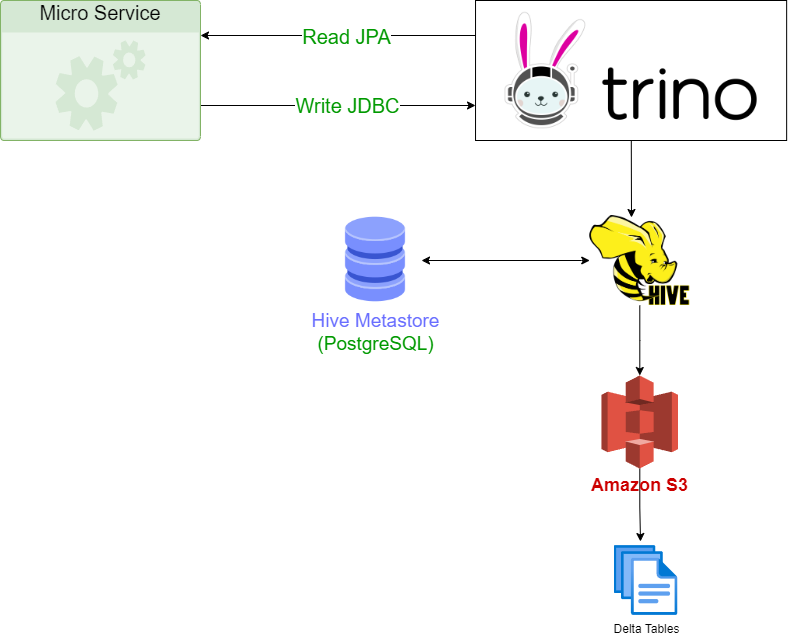
\includegraphics[width=\linewidth]{images/trino_microservice.png}
\caption{Architecture TRINO}\label{fig:arch-trino}
\end{figure}

\begin{figure}[H]
\centering
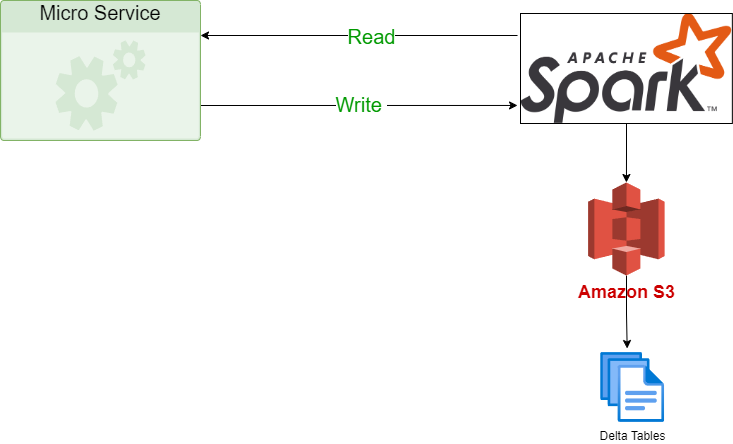
\includegraphics[width=\linewidth]{images/archi-spark.png}
\caption{Architecture SPARK}\label{fig:arch-spark}
\end{figure}
    
\subsection{Temps d'exécution}
\begin{enumerate}
    \item[$\bullet$] \textbf{Trino:} Trino est connu pour sa vitesse d'exécution élevée. Il utilise une architecture optimisée pour exécuter des requêtes SQL de manière très rapide, en exploitant la parallélisation et l'optimisation des requêtes. Trino peut fournir des temps d'exécution courts en ce qui concerne les requêtes sur Delta Lake.
    \item[$\bullet$] \textbf{Spark:} Spark est également conçu pour offrir des performances élevées, mais il peut nécessiter plus de temps pour lire les données à partir du disque. Cependant, Spark peut offrir des performances élevées lorsqu'il est utilisé avec des opérations de transformation complexes, grâce à son modèle de calcul distribué basé sur le disque.
\end{enumerate}

Nous avons effectué un test de performance sur une table Delta de 2 giga-octets en utilisant 2 ordinateurs:
\begin{enumerate}
    \item Le premier PC «DELL Latitude 5530» ou nous allons lancer les images Docker suivantes:
    \item \begin{enumerate}
        \item[$\bullet$] \textbf{Trino:} c’est l’image du serveur Trino pour l'interrogation de données distribué avec le langage SQL 
        \item[$\bullet$] \textbf{Hive:} Il sera utilisé conjointement avec Trino afin d’interroger et analyser des données stockées dans Hive grâce à la compatibilité entre les deux systèmes et le partage des métadonnées via le Hive Metastore.
        \item[$\bullet$] \textbf{PostgreSQL:} Il sera utilisé afin de stocker les métadonnées des tables Delta, des schémas et des partitions, facilitant ainsi la gestion, la découverte et l'accès aux données dans un environnement distribué. Il offre également des fonctionnalités d'optimisation des requêtes et de gestion des autorisations pour améliorer les performances et la sécurité des analyses de données.
        \item[$\bullet$] \textbf{AWS:} Où les delta tables sont trouvés.
    \end{enumerate}
    \item Le Dexième PC «ASUS ROG G752 VT» c’est là ou sera exécuté les micro-services springboot de SPARK et de TRINO.\@
\end{enumerate}

La configuration utilisée lors des tests est la suivante:
\begin{table}[h]
\centering
\label{tab:caracteristiques}
\begin{tabular}{|l|l|}
\hline
\textbf{Composant} & \textbf{Spécifications} \\ \hline
Processeur & 12th Gen Intel\textsuperscript{®} Core\textsuperscript{TM} i7-1255U 1.70 - 4.8 GHz \\ \hline
Fréquence processeur & 2.6 - 3.2 GHz \\ \hline
Mémoire vive & 24 GO \\ \hline
Type de mémoire vive & DDR4 \\ \hline
Puce graphique & Intel Iris Xe Graphics \\ \hline
Disque dur & 512GB PCIe NVMe Class 35 SSD \\ \hline
Type du système d'exploitation & Windows 11 64 bits \\ \hline
\end{tabular}
\caption{Caractéristiques techniques du PC « DEL Latitude 5530 »}
\end{table}

\begin{table}[h]
\centering
\label{tab:caracteristiques-2}
\begin{tabular}{|l|l|}
\hline
\textbf{Composant} & \textbf{Spécifications} \\ \hline
Processeur & Intel Core i7-6700HQ \\ \hline
Fréquence processeur & 2.6 - 3.2 GHz \\ \hline
Mémoire vive & 24 GO DDR4 \\ \hline
Disque dur & 1TO SSD + 1TO HDD \\ \hline
Type de mémoire vive & DDR4-SDRAM \\ \hline
Puce graphique & Nvidia GeForce GTX 970M \\ \hline
Quantité de mémoire graphique & 3072 Mo dédiée \\\hline
Type du système d'exploitation & Windows 10 64 bits \\ \hline
\end{tabular}
\caption{Caractéristiques techniques du PC «ASUS ROG G752 VT»}
\end{table}

Les résultats sont les suivants:

\begin{table}[h]
\centering
\label{tab:resultats}
\begin{tabular}{|l|l|l|}
\hline
\multirow{2}{*}{\textbf{Requêtes}} & \multicolumn{2}{c|}{\textbf{Implémentation}} \\ \cline{2-3}
& \textbf{Spark (s)} & \textbf{Trino (s)} \\ \hline
SELECT (par page et par limite de résultats par page - 100 par page) & 1.2 & 0.43 \\ \hline
Agrégation et regroupement & 2.1 & 0.8 \\ \hline
Tri & 2.2 & 0.8 \\ \hline
\end{tabular}
\caption{Caractéristiques techniques du PC «ASUS ROG G752 VT»}
\end{table}

\subsection{Gestion de la mémoire}
\begin{enumerate}
    \item[$\bullet$] \textbf{Trino:} Trino utilise principalement la mémoire pour accélérer le traitement des requêtes. Il dispose d'un moteur de requêtage en mémoire qui optimise l'accès aux données et minimise les temps d'accès. Cependant, cela signifie que Trino peut nécessiter une quantité de mémoire significative pour traiter de grands ensembles de données.
    \item[$\bullet$] \textbf{Spark:} Spark utilise un modèle de calcul distribué basé sur le disque, ce qui signifie que les données sont généralement stockées sur le disque et chargées en mémoire selon les besoins. Cela permet à Spark de gérer des ensembles de données beaucoup plus volumineux que ce qui peut tenir en mémoire.
\end{enumerate}
    
\subsection{Écosystème et intégrations}
\begin{enumerate}
    \item[$\bullet$] \textbf{Trino:} Trino dispose d'un écosystème en pleine croissance avec une large gamme de connecteurs et d'intégrations, ce qui permet d'accéder à différentes sources de données, y compris Delta Lake. Il est compatible avec divers outils de visualisation et de traitement des données.
    \item[$\bullet$] \textbf{Spark:} Spark est un projet mature avec un écosystème riche d'outils, de bibliothèques et de connecteurs. Il bénéficie d'une large communauté de développeurs et de nombreuses ressources d'apprentissage. Spark prend également en charge le traitement de données en continu et le traitement par lots.
\end{enumerate}

\subsection{Évolutivité}
\begin{enumerate}
    \item[$\bullet$] \textbf{Trino:} Trino est conçu pour être hautement évolutif et peut gérer de grands ensembles de données. Il peut être facilement configuré pour s'adapter à des charges de travail intensives et à des volumes de données importants.
    \item[$\bullet$] \textbf{Spark:} Spark est également conçu pour l'évolutivité et peut traiter des ensembles de données massifs. Il dispose d'un système de traitement distribué qui peut s'adapter à différentes configurations de clusters et de ressources.
\end{enumerate}

\subsection{Support des fonctionnalités Delta Lake}
\begin{enumerate}
    \item[$\bullet$] \textbf{Trino:} Trino dispose d'un connecteur officiel pour Delta Lake, ce qui lui permet de lire et d'écrire des données dans Delta Lake. Il prend en charge les fonctionnalités essentielles de Delta Lake, telles que la gestion des transactions ACID, les mises à jour incrémentielles et les opérations de fusion ("merge").
    \item[$\bullet$] \textbf{Spark:} Spark dispose également d'un support intégré pour Delta Lake. Il offre des fonctionnalités avancées de gestion des données Delta, notamment la prise en charge des transactions ACID, des opérations de fusion performantes et des mécanismes de contrôle de version des données.
\end{enumerate}

\subsection{Facilité d'utilisation}
\begin{enumerate}
    \item[$\bullet$] \textbf{Trino:} Trino offre une interface SQL standard, ce qui facilite son utilisation pour les utilisateurs familiers avec SQL. Il propose également des outils de requêtage interactif conviviaux et des options de configuration flexibles.
    \item[$\bullet$] \textbf{Spark:} Spark propose une interface SQL via Spark SQL, mais il est également orienté vers le traitement de données par le biais d'un API plus large. Spark peut être plus complexe à utiliser pour les utilisateurs moins familiers avec les concepts du traitement distribué.
\end{enumerate}

\subsection{Autres statistiques}

\begin{longtable}{|p{0.23\linewidth}|p{0.35\linewidth}|p{0.42\linewidth}|}
\hline
\textbf{} & \textbf{Spark} & \textbf{Trino} \\ \hline
\textbf{Expérience \newline Développeur} & 

\includegraphics[width=0.28in,height=0.28in]{images/image3.png}
\includegraphics[width=0.28in,height=0.28in]{images/image3.png}\newline
La syntaxe de Spark exige que les PME aient une expérience en ingénierie de données &

\includegraphics[width=0.28in,height=0.28in]{images/image3.png}
\includegraphics[width=0.28in,height=0.28in]{images/image3.png}
\includegraphics[width=0.28in,height=0.28in]{images/image3.png}\newline
Une interface SQL standard, ce qui facilite son utilisation pour les utilisateurs familiers avec SQL \\ \hline
\textbf{Coût} & 
Équipe: 
\includegraphics[width=0.33in,height=0.35in]{images/image4.jpg}
\includegraphics[width=0.33in,height=0.35in]{images/image4.jpg}\newline
Infrastructure: \textcolor[RGB]{0, 128, 0}{\textbf{\large \$}} & 
Équipe: 
\includegraphics[width=0.33in,height=0.35in]{images/image4.jpg}
\includegraphics[width=0.33in,height=0.35in]{images/image4.jpg}\newline
Infrastructure: \textcolor[RGB]{0, 128, 0}{\textbf{\large \$}} \\ \hline
\textbf{Fiabilité} & 

\includegraphics[width=0.28in,height=0.28in]{images/image3.png}
\includegraphics[width=0.28in,height=0.28in]{images/image3.png}
\includegraphics[width=0.28in,height=0.28in]{images/image3.png}\newline
Produit mature maintenu en interne et pris en charge par Google Dataproc &

\includegraphics[width=0.28in,height=0.28in]{images/image3.png}
\includegraphics[width=0.28in,height=0.28in]{images/image3.png}\newline
A été en panne à quelques reprises car l'équipe interne apprend à maintenir et à évoluer \\ \hline
\textbf{Caractéristiques et Open sources} & 

\includegraphics[width=0.28in,height=0.28in]{images/image3.png}
\includegraphics[width=0.28in,height=0.28in]{images/image3.png}
\includegraphics[width=0.28in,height=0.28in]{images/image3.png}\newline
A été soutenu par la communauté open source depuis 2014 &

\includegraphics[width=0.28in,height=0.28in]{images/image3.png}
\includegraphics[width=0.28in,height=0.28in]{images/image3.png}
\includegraphics[width=0.28in,height=0.28in]{images/image3.png}\newline
A été soutenu par la communauté open source depuis 2019. Shopify a apporté des contributions. \\ \hline
\textbf{Usage} & 
\textasciitilde800,000 emplois/jour & 
3000 utilisateurs actifs/semaine \newline
\textasciitilde200,000 requêtes/semaine \\ \hline
\end{longtable}

\section{Schématisation de la Solution}

Dans le cadre de la schématisation de la solution, nous avons opté pour une architecture basée sur des microservices, utilisant les technologies suivantes : Spring Data, JPA, Hibernate, JDBC et Trino.

Les microservices sont développés en utilisant Spring Data, qui fournit une abstraction de haut niveau pour interagir avec la base de données. Cela permet d'utiliser des annotations et des interfaces pour définir les entités, les requêtes et les opérations de persistance. JPA (Java Persistence API) est utilisé comme couche d'interface pour interagir avec la base de données, tandis que Hibernate est utilisé comme fournisseur de persistance, permettant la gestion des objets Java et leur mapping vers Trino.

La communication entre les microservices est assurée par un broker Kafka. Kafka est une plateforme de streaming distribuée qui permet aux microservices d'échanger des messages en temps réel. Les microservices publient des événements sur des sujets Kafka, et d'autres microservices peuvent s'abonner à ces sujets pour recevoir les événements correspondants.

Pour gérer l'authentification et l'autorisation, nous utilisons Spring Cloud Gateway. Ce composant reçoit les appels de services provenant des applications Web, mobiles ou de bureau. Ces applications envoient un jeton JWT (JSON Web Token) à Spring Cloud Gateway pour authentification. Ce dernier vérifie la disponibilité du jeton en contactant Keycloak, qui est responsable de la gestion des identités et des accès. Une fois le jeton validé, Spring Cloud Gateway autorise la demande à passer vers les microservices.

Les microservices communiquent avec Trino en utilisant le connecteur JDBC\@. Trino est responsable de l'interrogation et du traitement des données sur une grande quantité de sources de données. Il stocke les métadonnées dans Hive, qui est un entrepôt de données basé sur Hadoop. Trino utilise également le concept de tables Delta pour gérer les modifications incrémentielles des données. Ces tables Delta sont stockées sur AWS (Amazon Web Services), offrant une solution de stockage évolutive et fiable.

\begin{figure}[H]
\centering
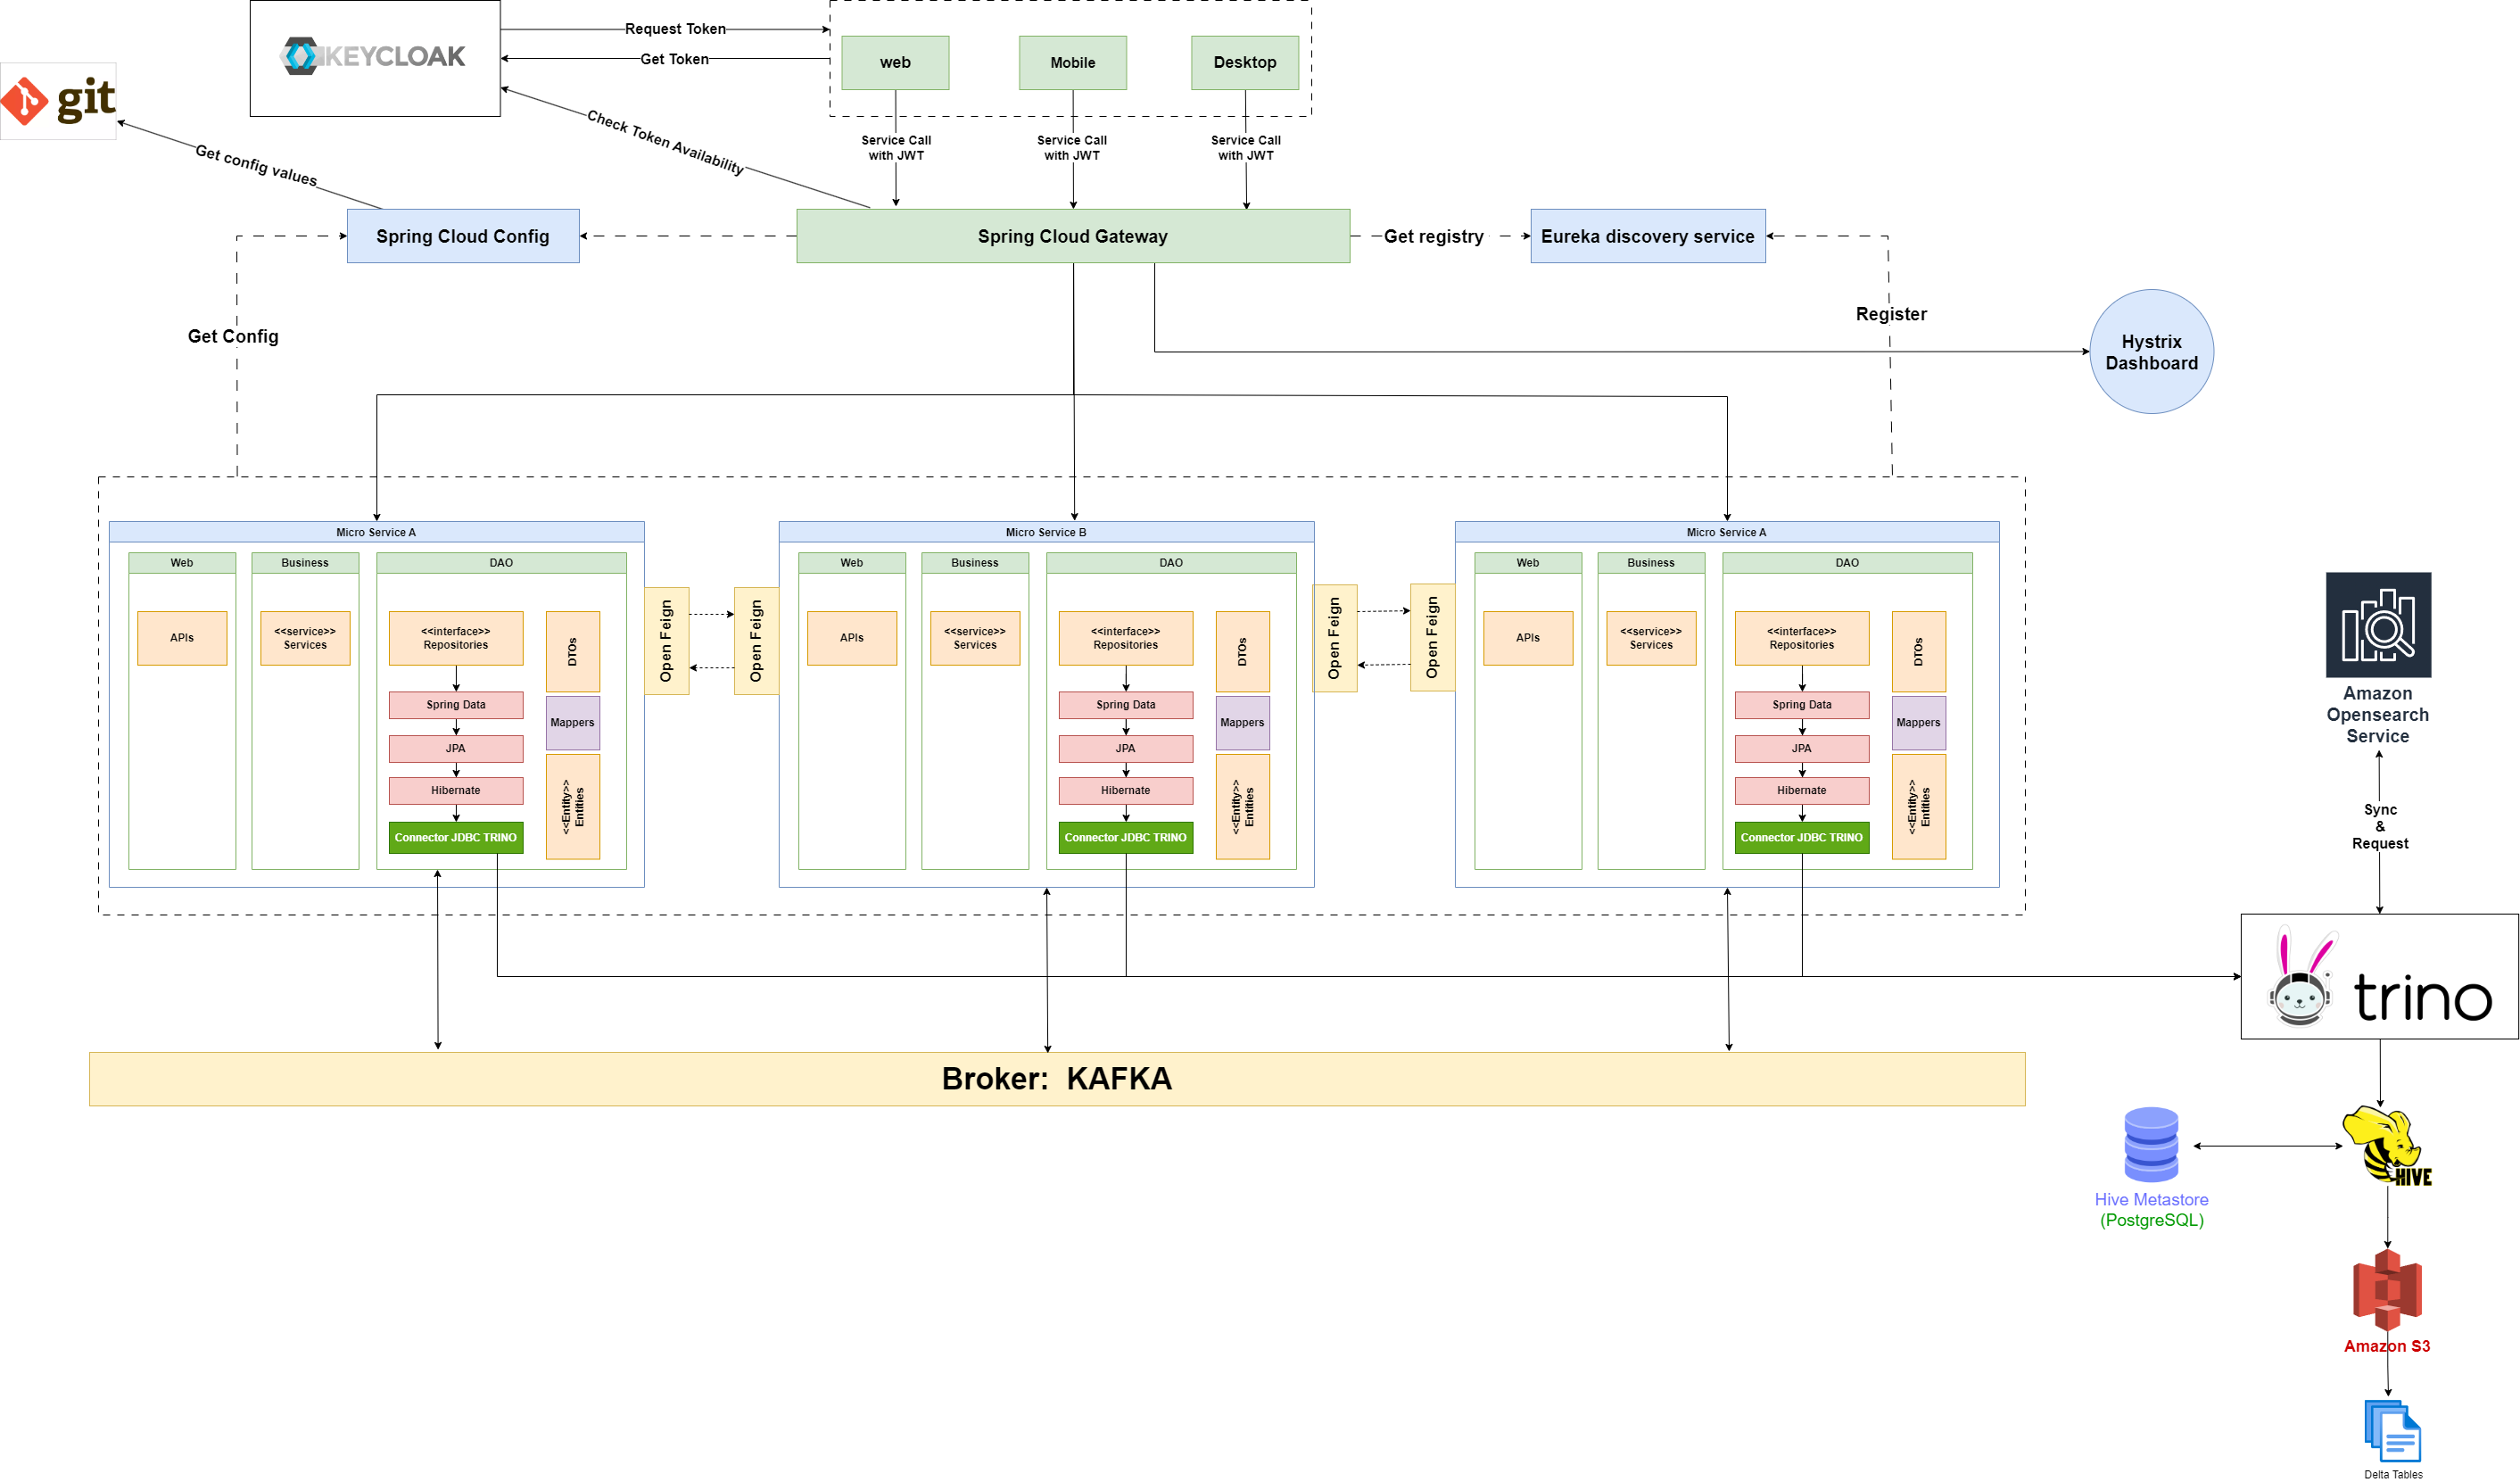
\includegraphics[width=\linewidth]{images/architecture-solution.png}
\caption{Architecture de solution}\label{fig:solution}
\end{figure}

\section{Avantages}

L'architecture que nous avons choisie présente plusieurs avantages significatifs:

\begin{enumerate}
    \item[$\bullet$] \textbf{Évolutivité:} L'architecture basée sur des microservices permet une évolutivité horizontale, ce qui signifie que chaque microservice peut être déployé et mis à l'échelle indépendamment en fonction de ses besoins spécifiques. Cela permet d'ajuster la capacité et les ressources de manière granulaire, ce qui facilite la gestion des charges de travail élevées et l'adaptation aux besoins croissants de l'application.
    \item[$\bullet$] \textbf{Modularité:} La conception modulaire des microservices permet une gestion plus efficace du développement, du déploiement et de la maintenance. Chaque microservice peut être développé indépendamment, ce qui facilite la collaboration entre les équipes et favorise la réutilisation du code. De plus, les modifications ou les mises à jour apportées à un microservice n'ont pas d'impact sur les autres, ce qui réduit les risques d'erreurs et de conflits. 
    \item[$\bullet$] \textbf{Flexibilité technologique:} Les microservices offrent une flexibilité en termes de choix technologiques. Chaque microservice peut être développé en utilisant les technologies les plus adaptées à sa fonctionnalité spécifique. Cela permet d'exploiter au mieux les avantages de chaque technologie et de choisir les outils les mieux adaptés à chaque composant de l'architecture. 
    \item[$\bullet$] \textbf{Communication efficace:} L'utilisation de Kafka comme broker de streaming facilite la communication entre les microservices. Kafka garantit la fiabilité et la scalabilité des échanges d'événements en temps réel, ce qui permet une communication fluide et une synchronisation efficace entre les différents composants du système. 
    \item[$\bullet$] \textbf{Sécurité renforcée:} L'intégration de Keycloak pour l'authentification et l'autorisation offre un niveau élevé de sécurité. Les jetons JWT sont utilisés pour l'identification des utilisateurs, et Spring Cloud Gateway assure la vérification et la gestion de ces jetons. Cela garantit que seules les personnes autorisées ont accès aux ressources et aux fonctionnalités appropriées, renforçant ainsi la sécurité de l'application.
    \item[$\bullet$] \textbf{Performances optimisées:}  L'utilisation de Trino comme moteur de requête distribué permet d'interroger et de traiter de grandes quantités de données de manière parallèle et efficace. Trino offre des performances élevées et une optimisation des requêtes, ce qui permet d'obtenir des résultats plus rapidement et d'améliorer l'expérience utilisateur. 
\end{enumerate}

\section{Visualisation}

Dans cette section, nous présenterons des captures d'écran des différents microservices de notre solution, notamment Swagger pour l'API, la console de Trino pour l'exploration des données et le site web d'Izicap. Ces captures d'écran illustreront l'interface utilisateur et les fonctionnalités offertes par chaque service.
\subsection{Console de Trino}

\begin{figure}[H]
\centering
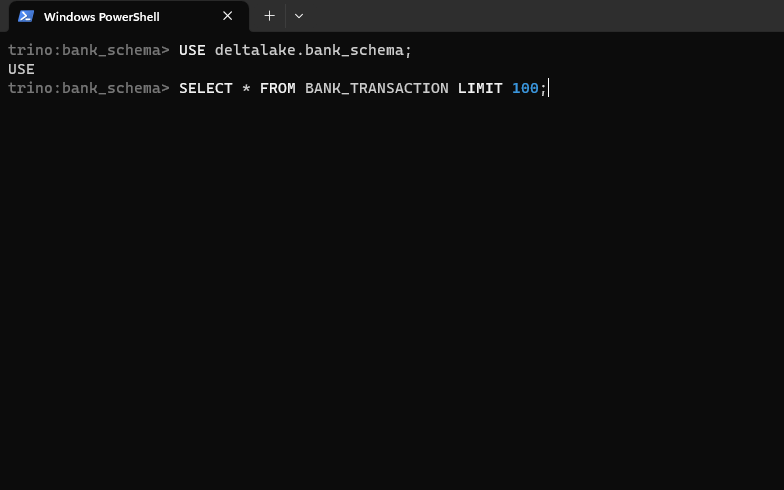
\includegraphics[width=\linewidth]{images/trino-1.png}
\caption{Console Trino}\label{fig:trino-1}
\end{figure}

\begin{figure}[H]
\centering
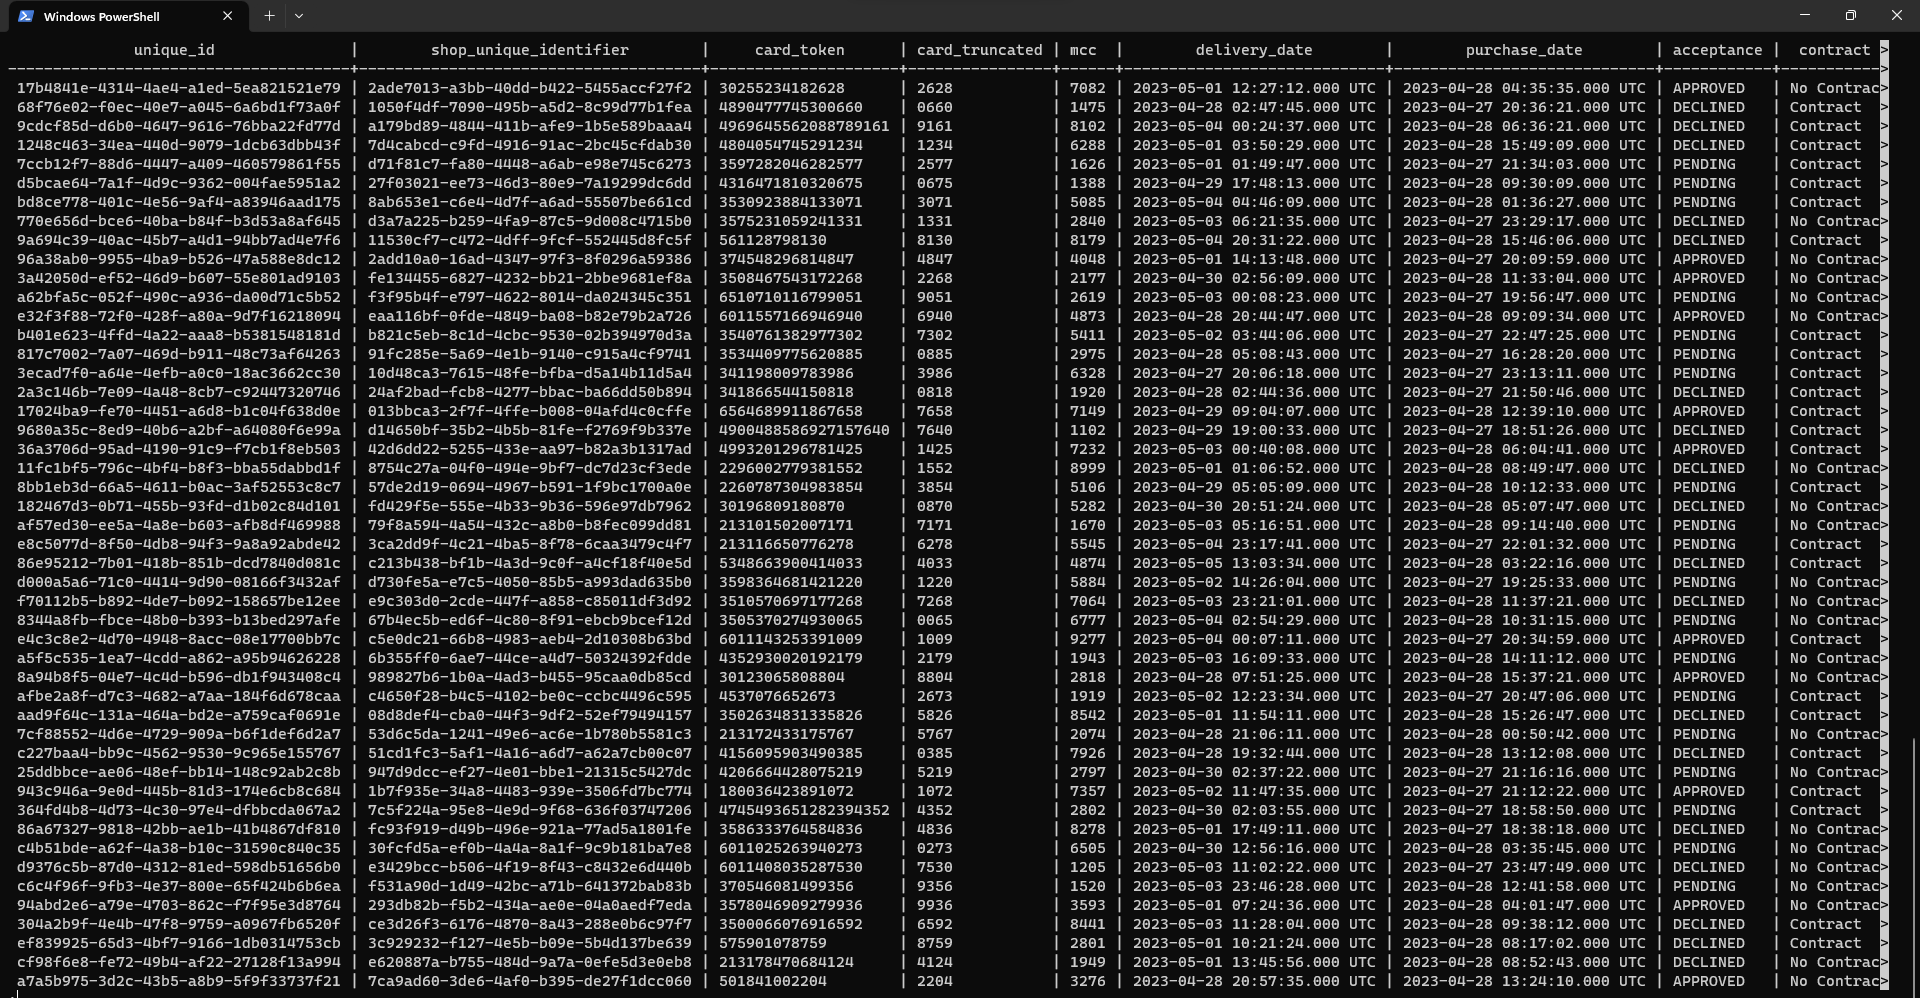
\includegraphics[width=\linewidth]{images/trino-2.png}
\caption{Console Trino SELECT}\label{fig:trino-2}
\end{figure}

\begin{figure}[H]
\centering
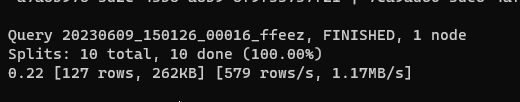
\includegraphics[width=\linewidth]{images/trino-3.png}
\caption{Console Trino}\label{fig:trino-3}
\end{figure}

Ces captures d'écran de la console de Trino met en évidence l'interface de requêtes de données avancée fournie par Trino. Les développeurs et les analystes peuvent exécuter des requêtes SQL sur les données stockées dans Trino, explorer les schémas, prévisualiser les résultats et effectuer des opérations analytiques pour extraire des informations précieuses.

\subsection{Micro services}
\begin{figure}[H]
\centering
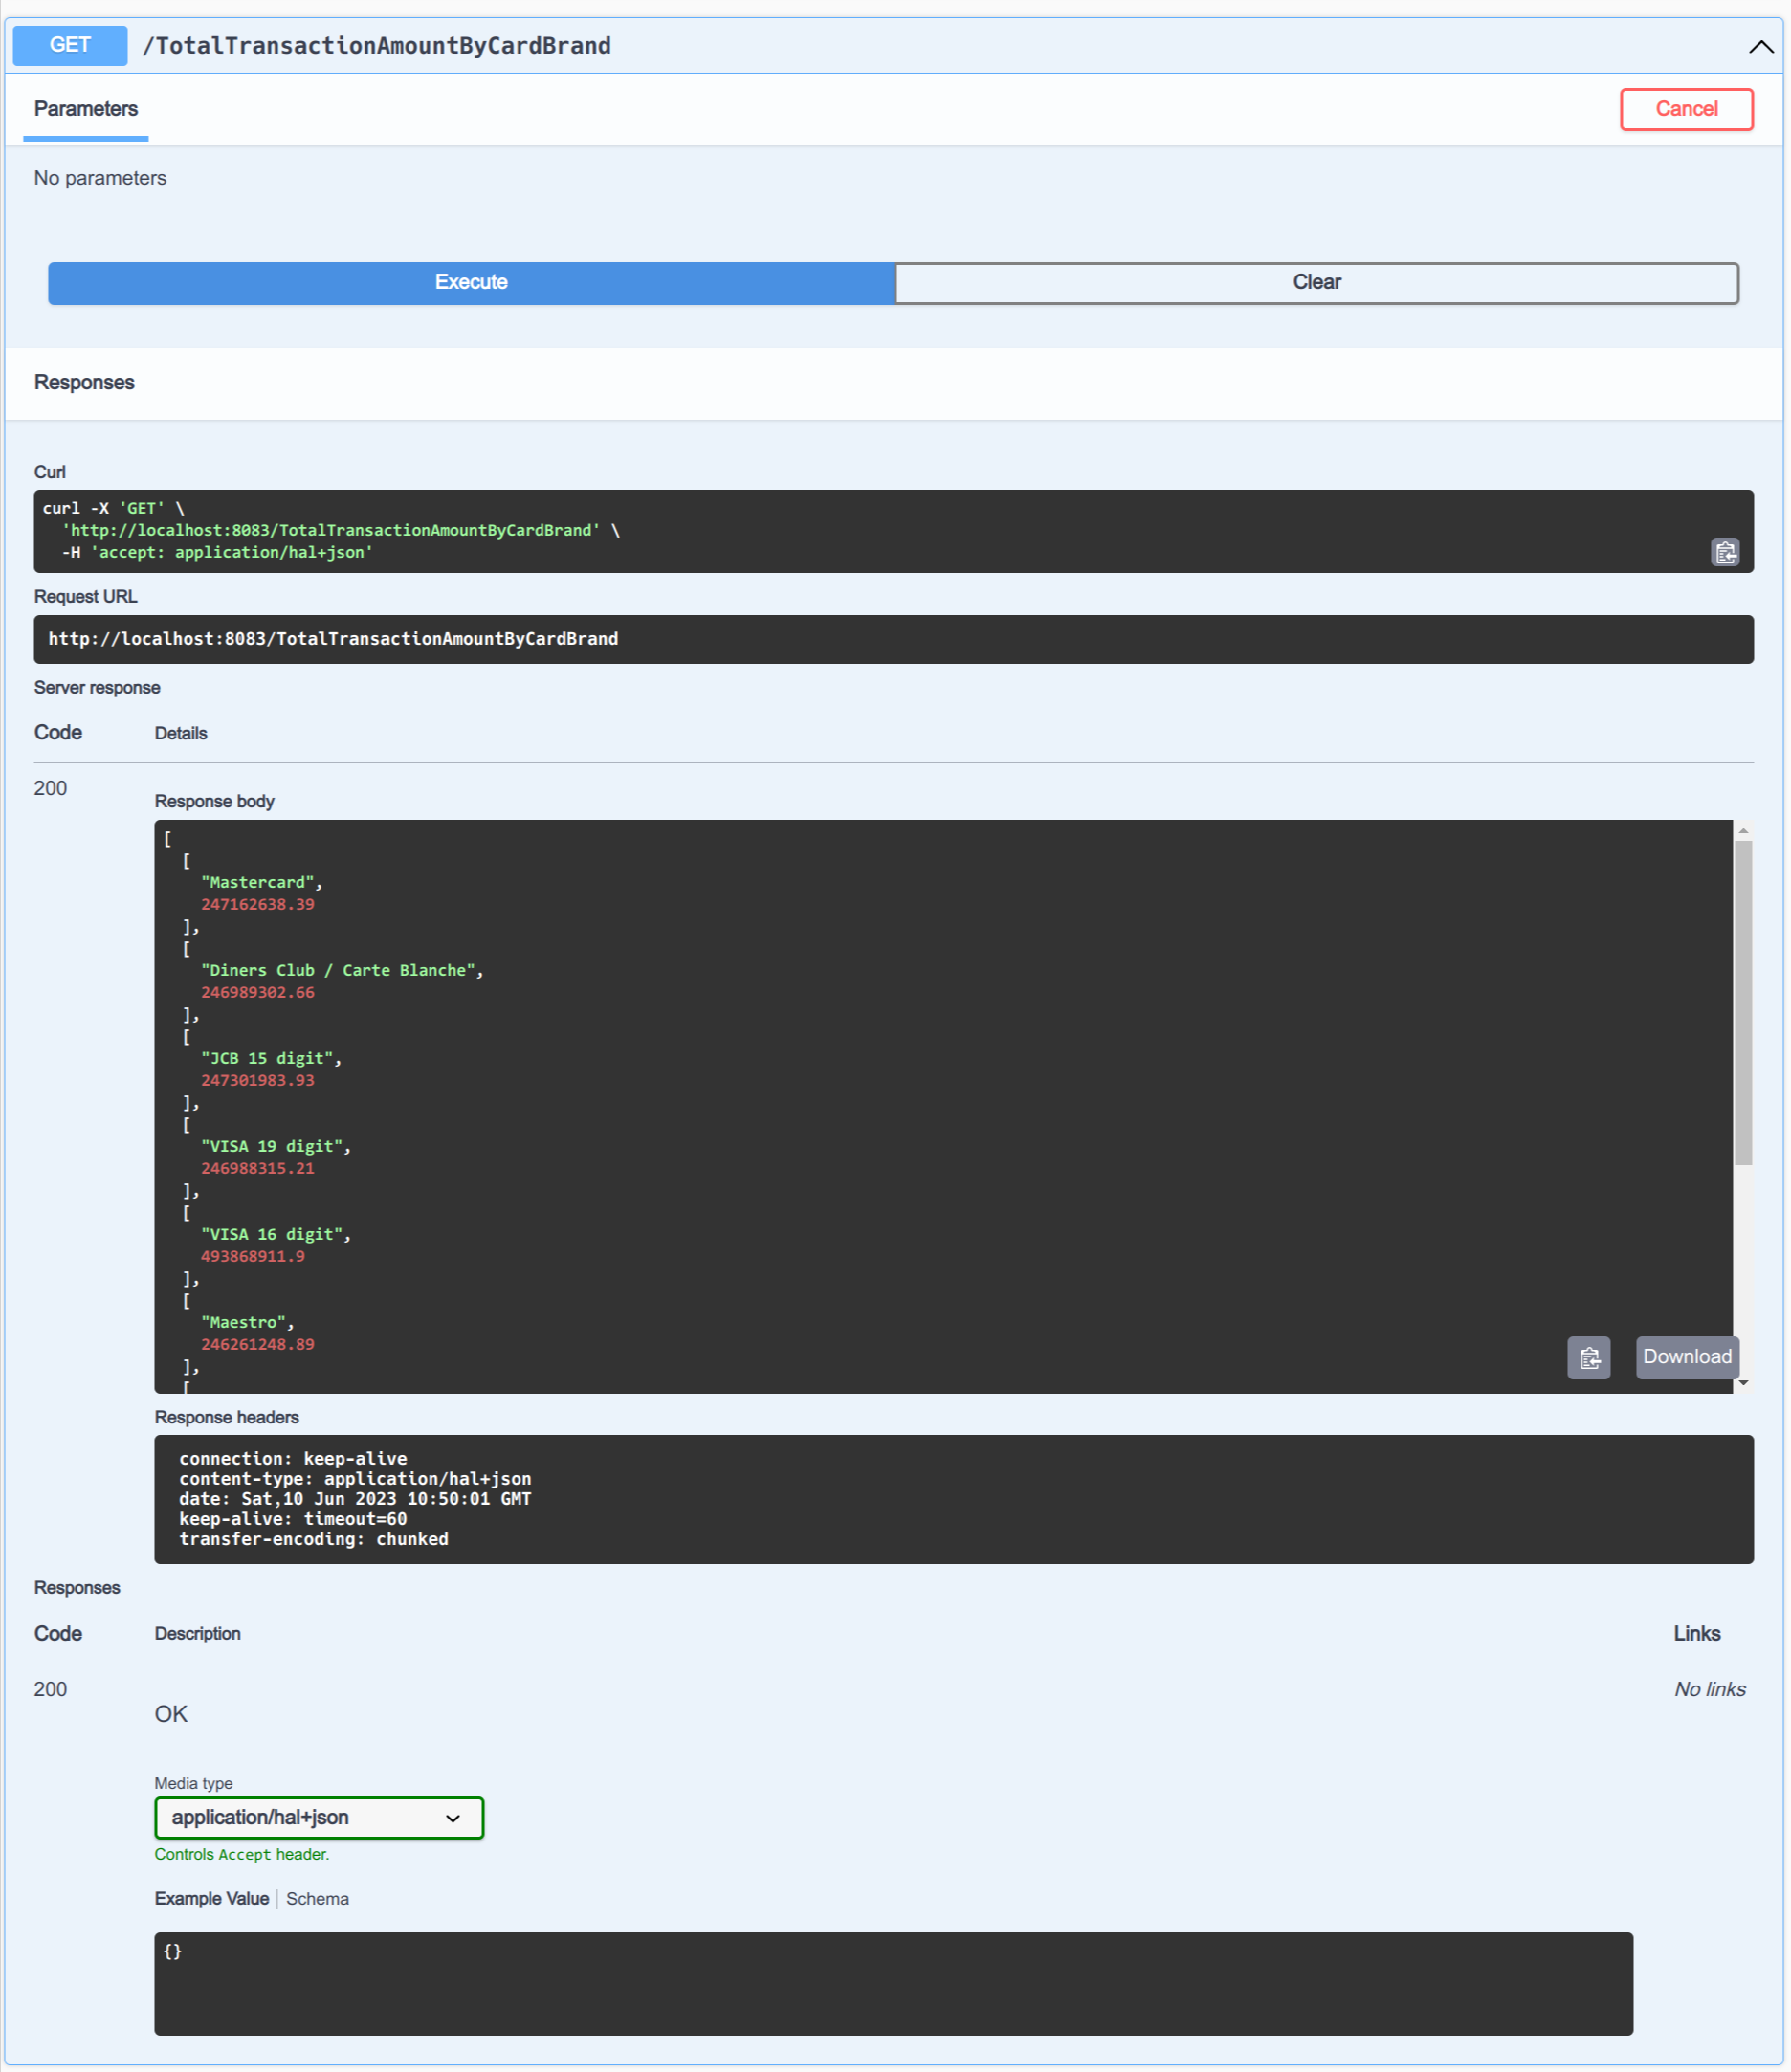
\includegraphics[width=\linewidth]{images/Swagger-UI-1.png}
\caption{Swagger UI}\label{fig:swagger-1}
\end{figure}

\begin{figure}[H]
\centering
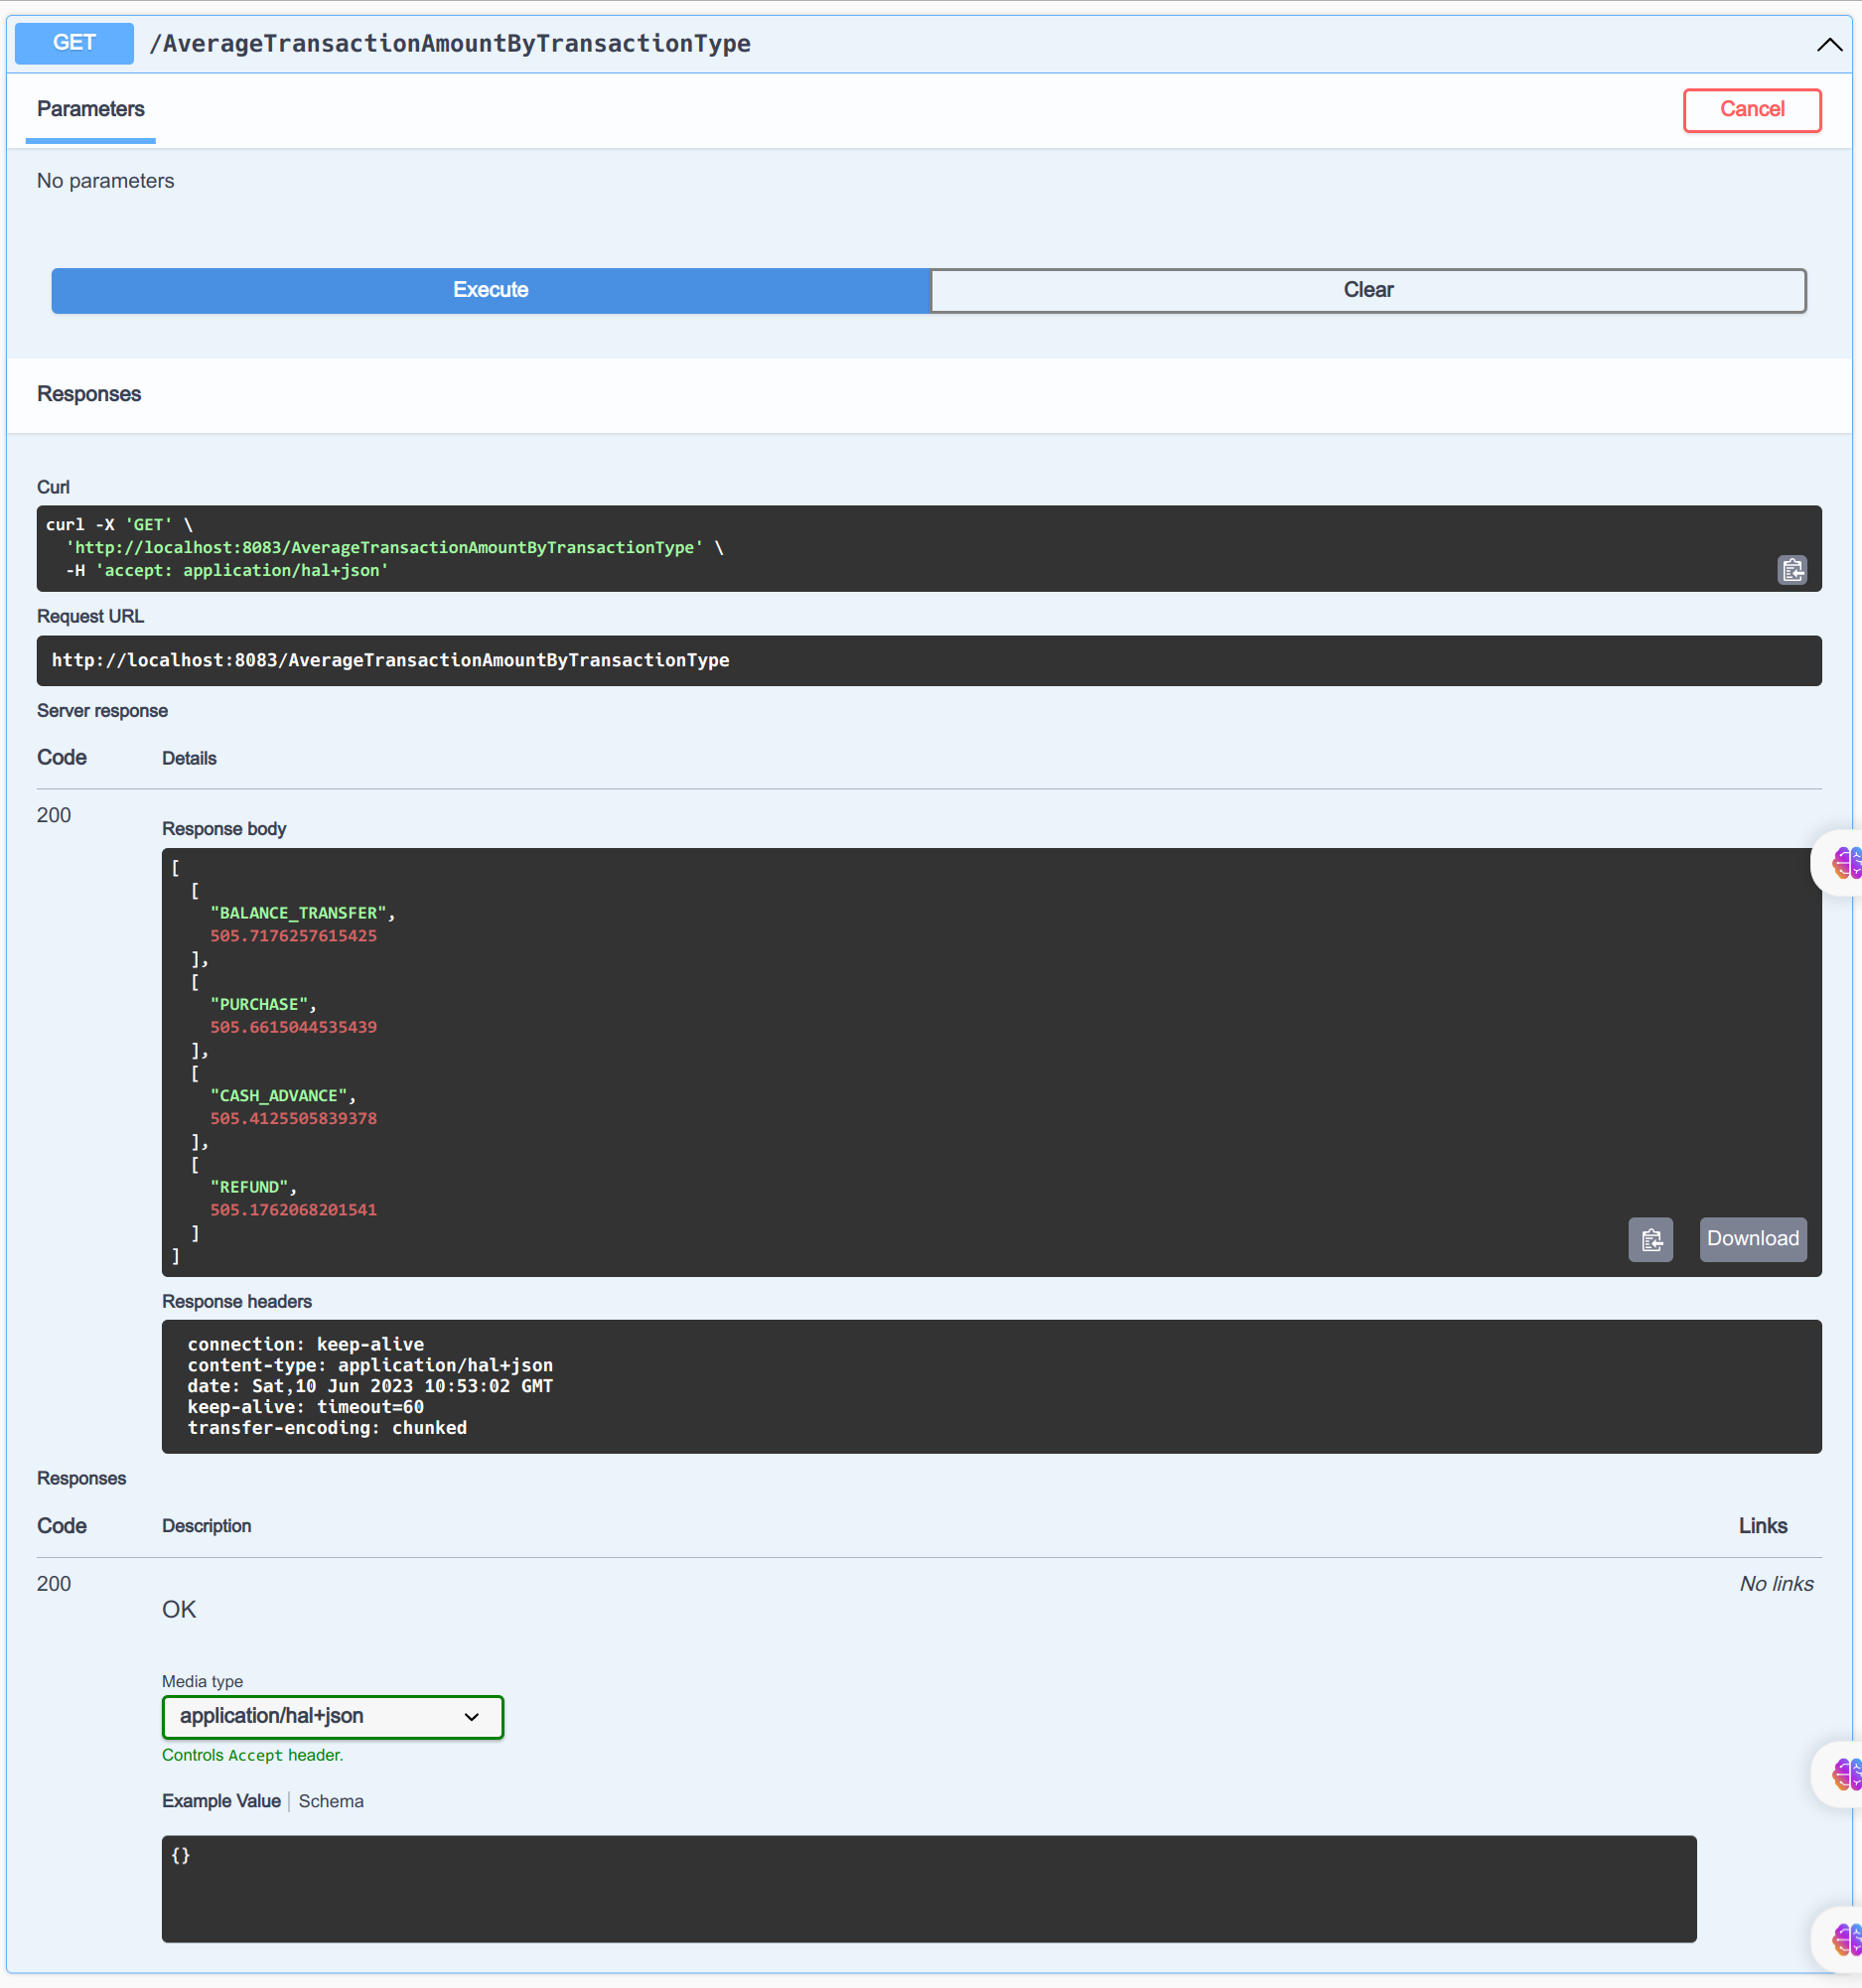
\includegraphics[width=\linewidth]{images/Swagger-UI-2.png}
\caption{Swagger UI}\label{fig:swagger-2}
\end{figure}

\begin{figure}[H]
\centering
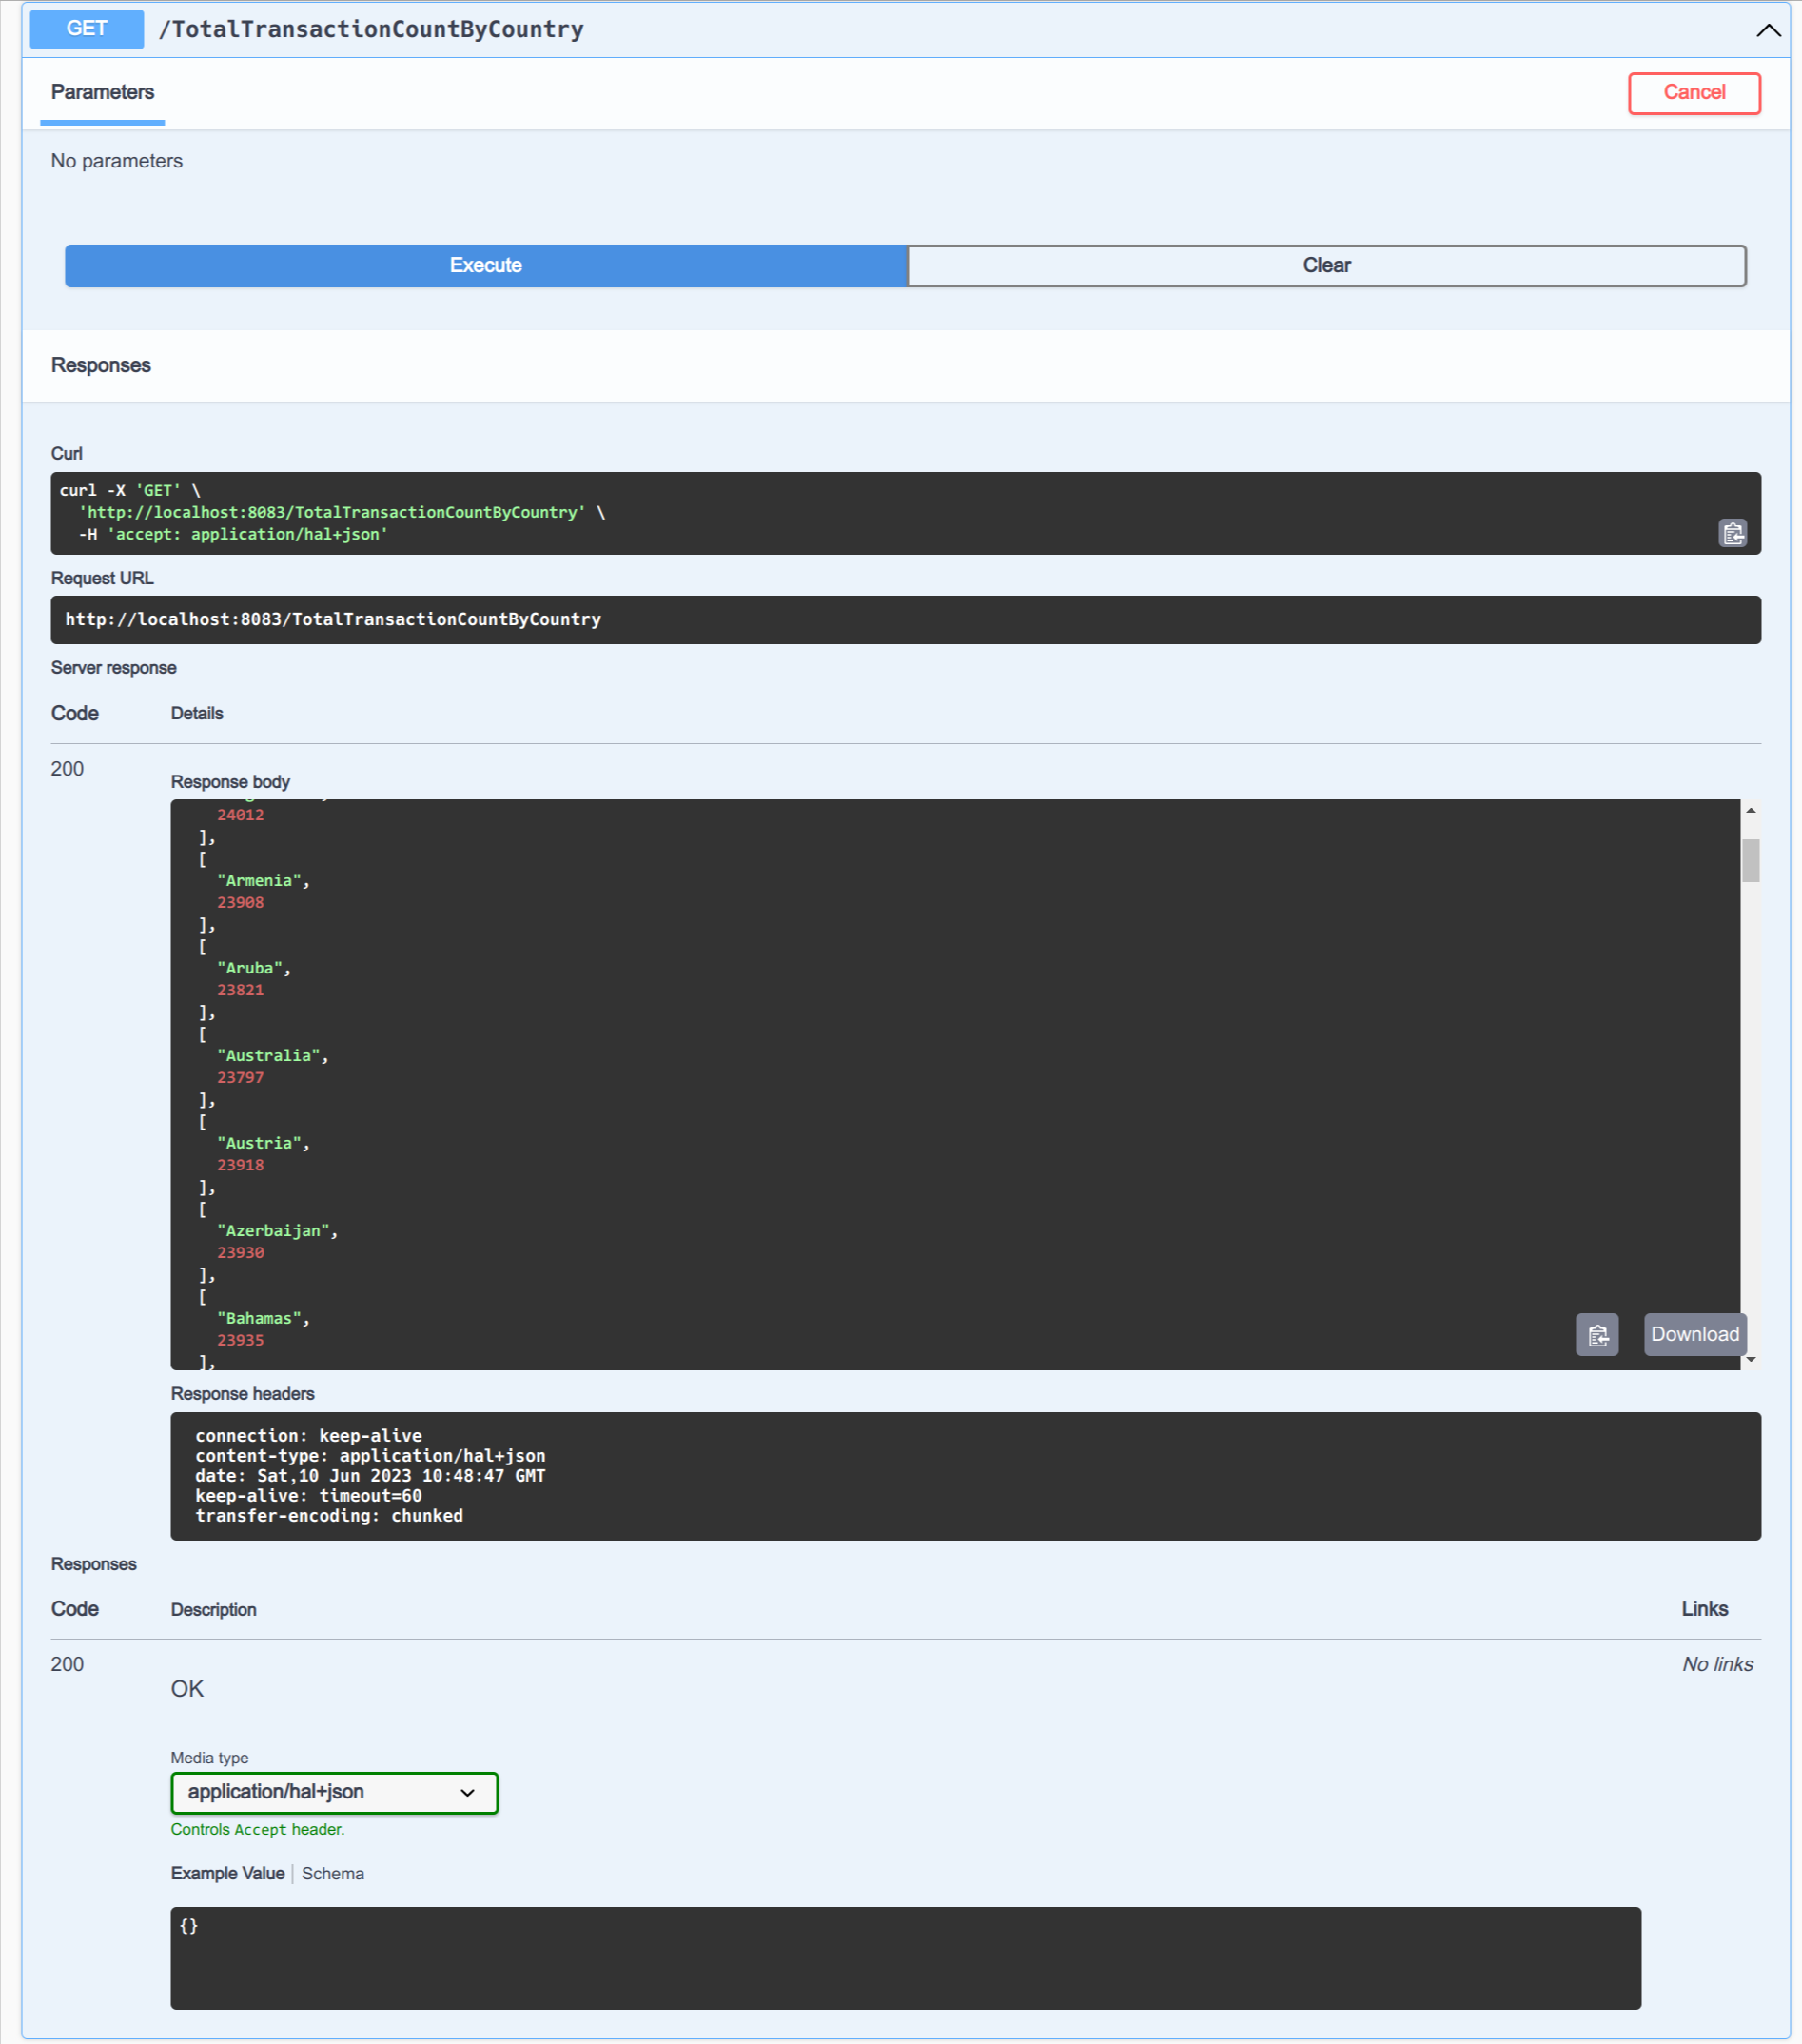
\includegraphics[width=\linewidth]{images/Swagger-UI.png}
\caption{Swagger UI}\label{fig:swagger-3}
\end{figure}

\begin{figure}[H]
\centering
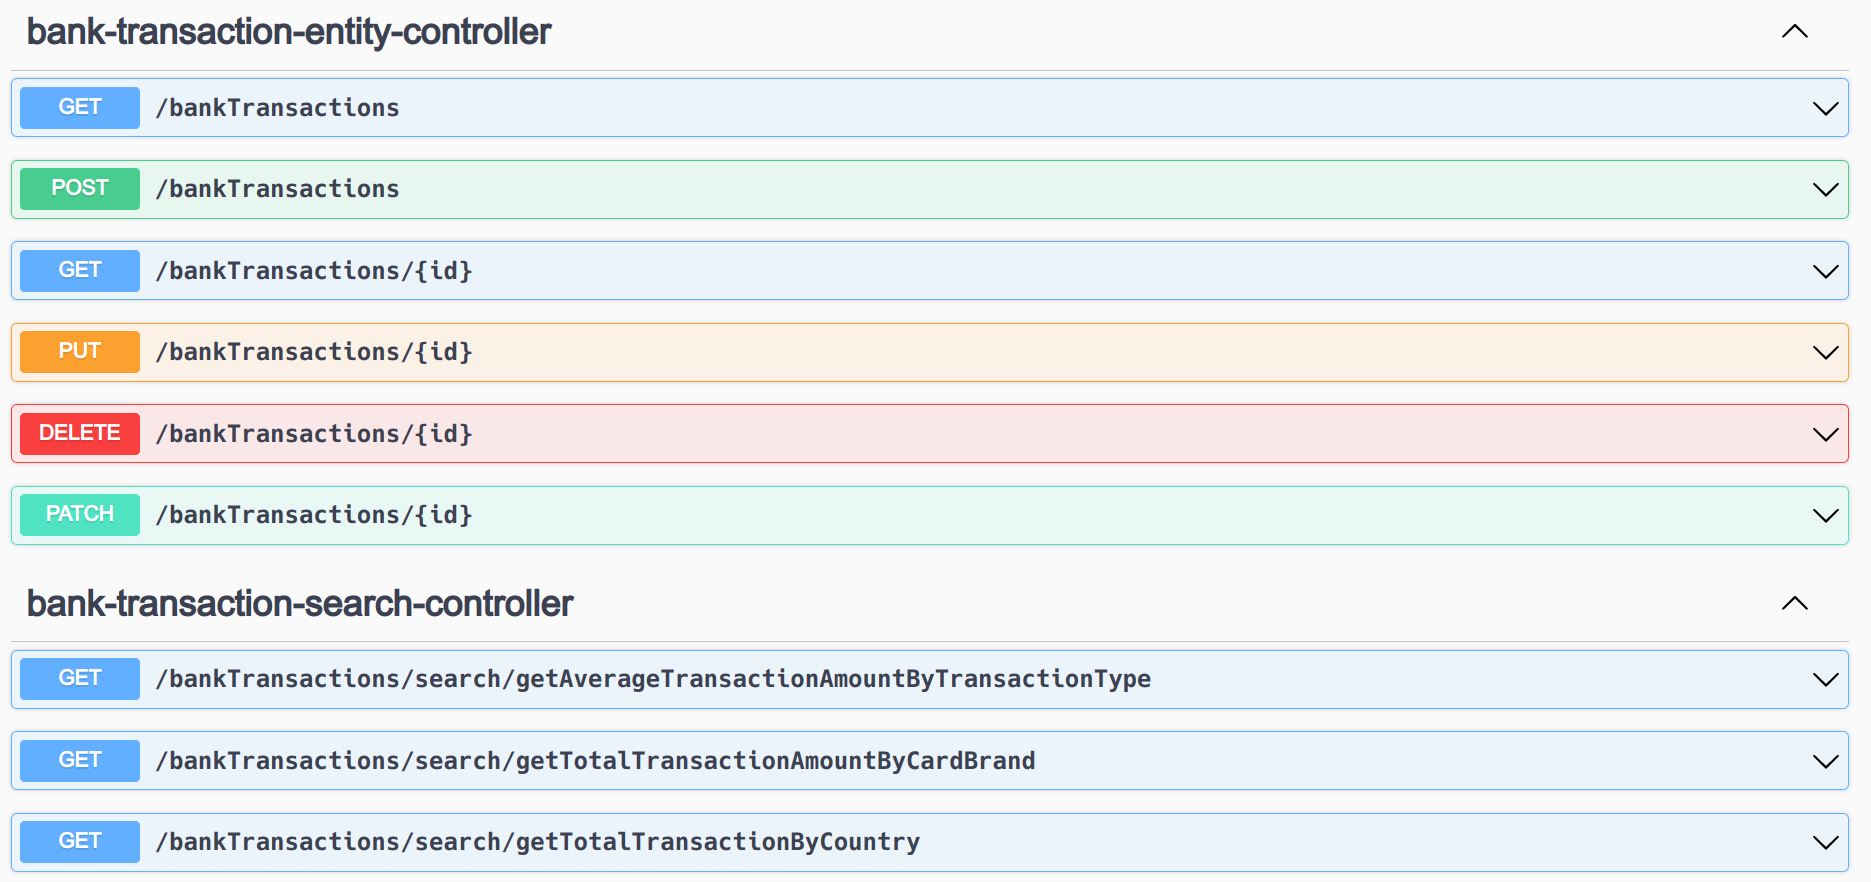
\includegraphics[width=\linewidth]{images/Swagger-UI-3.png}
\caption{Swagger UI}\label{fig:swagger-4}
\end{figure}

Ces images montrent la documentation détaillée de notre API à l'aide de Swagger. Cette interface conviviale permet aux développeurs de comprendre les endpoints disponibles, les paramètres requis, les réponses attendues et les exemples d'utilisation. Swagger facilite l'intégration et la communication avec nos microservices.

\subsection{Delta Lake}

\begin{figure}[H]
\centering
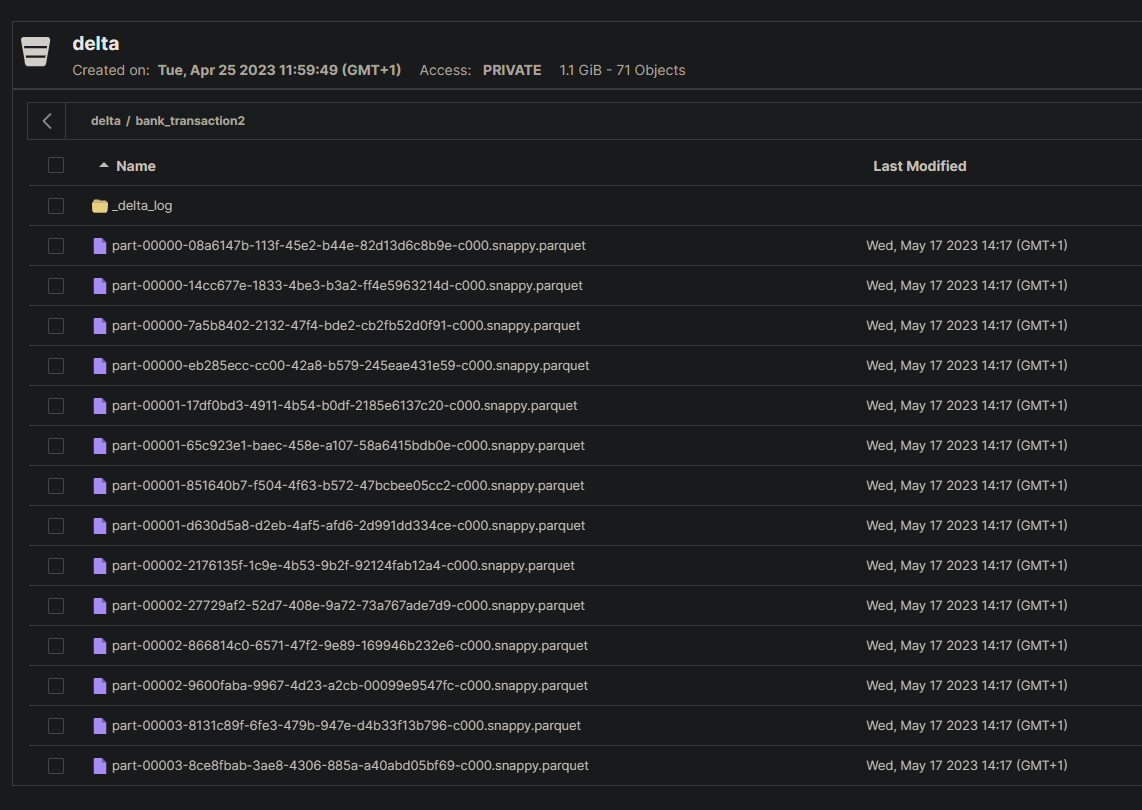
\includegraphics[width=\linewidth]{images/delta-lake-dossier.png}
\caption{Parquet Data}\label{fig:delta-lake-dossier}
\end{figure}

Nous avons les fichiers de données au format Parquet. Les fichiers Parquet sont optimisés pour le stockage et la récupération efficaces des données. Ils sont compressés et structurés de manière à permettre des requêtes rapides et une lecture sélective des données. Ces fichiers Parquet contiennent les données réelles de la table, organisées en colonnes et partitions, ce qui facilite la manipulation et l'analyse ultérieure des données.    

\subsection{UI Izicap}

\begin{figure}[H]
\centering
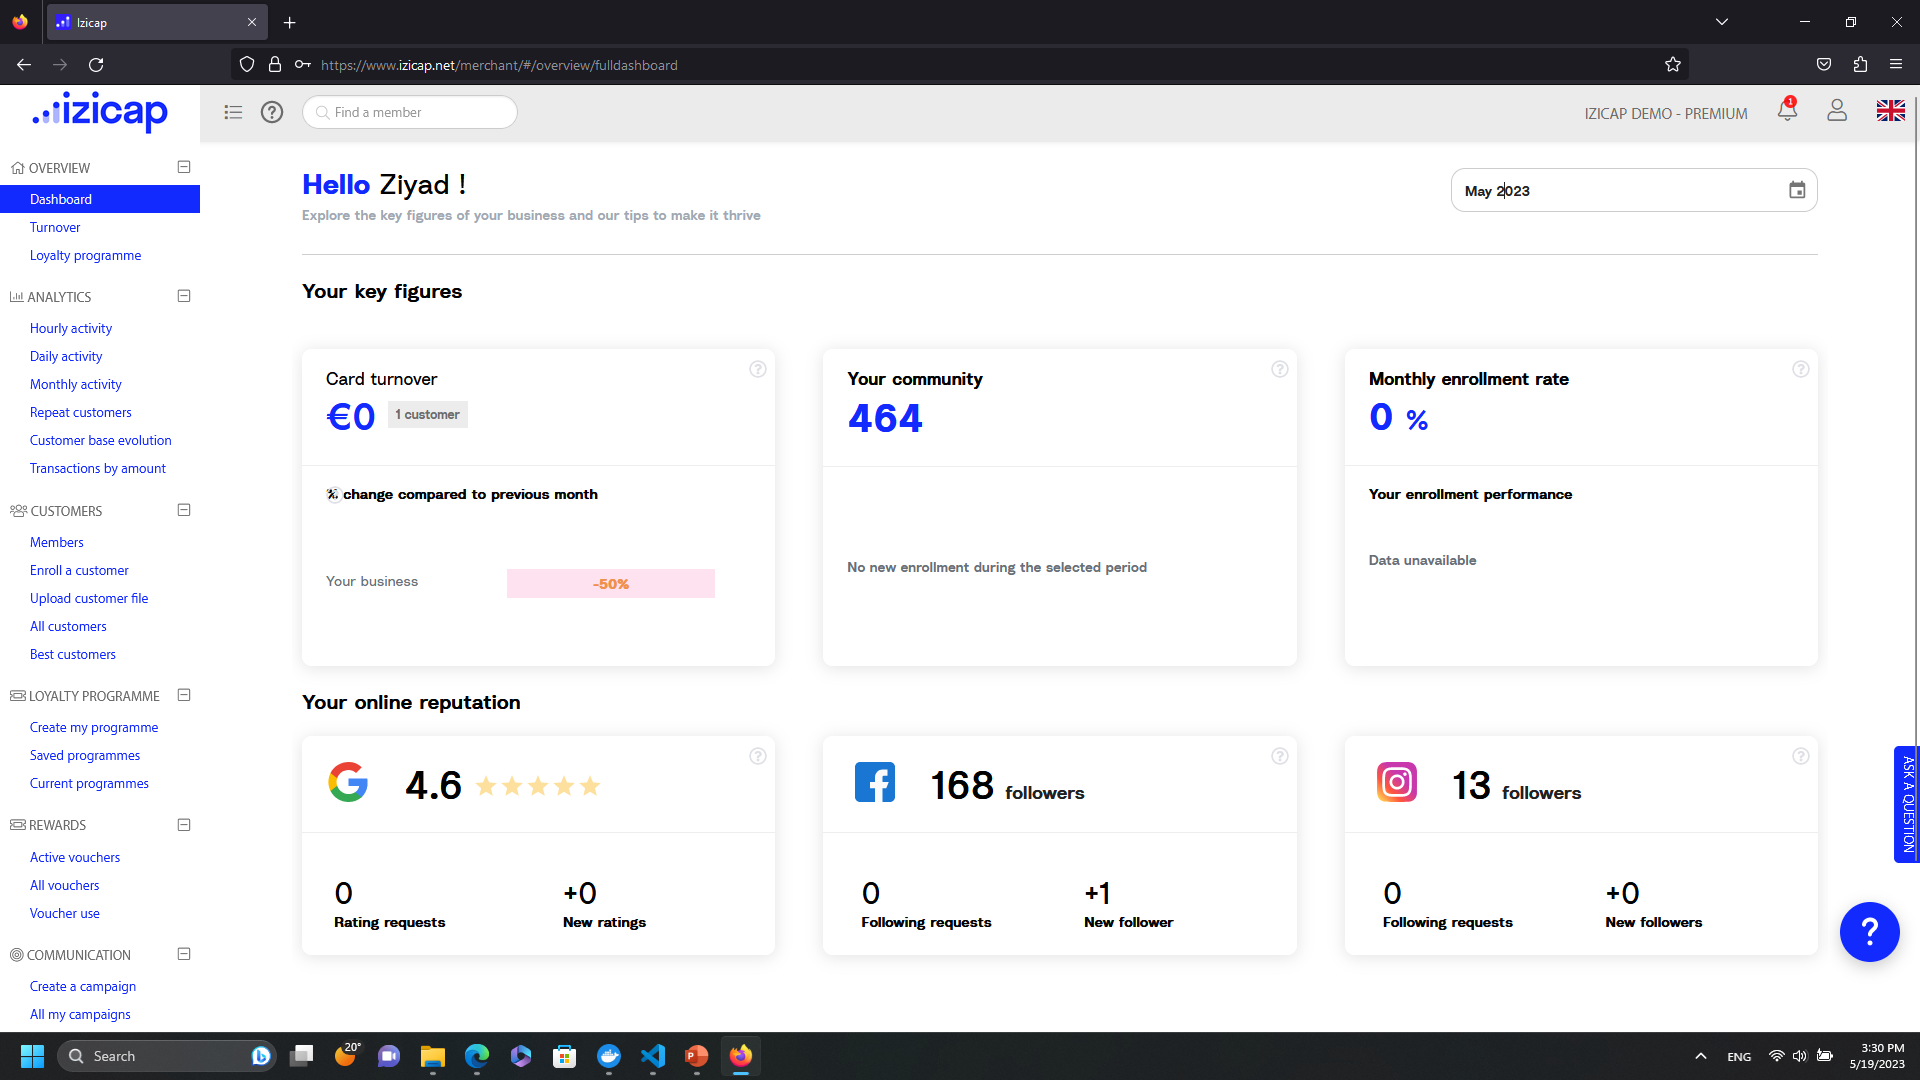
\includegraphics[width=\linewidth]{images/izicap-portail.png}
\caption{Portail Izicap}\label{fig:izicap-1}
\end{figure}


\begin{figure}[H]
\centering
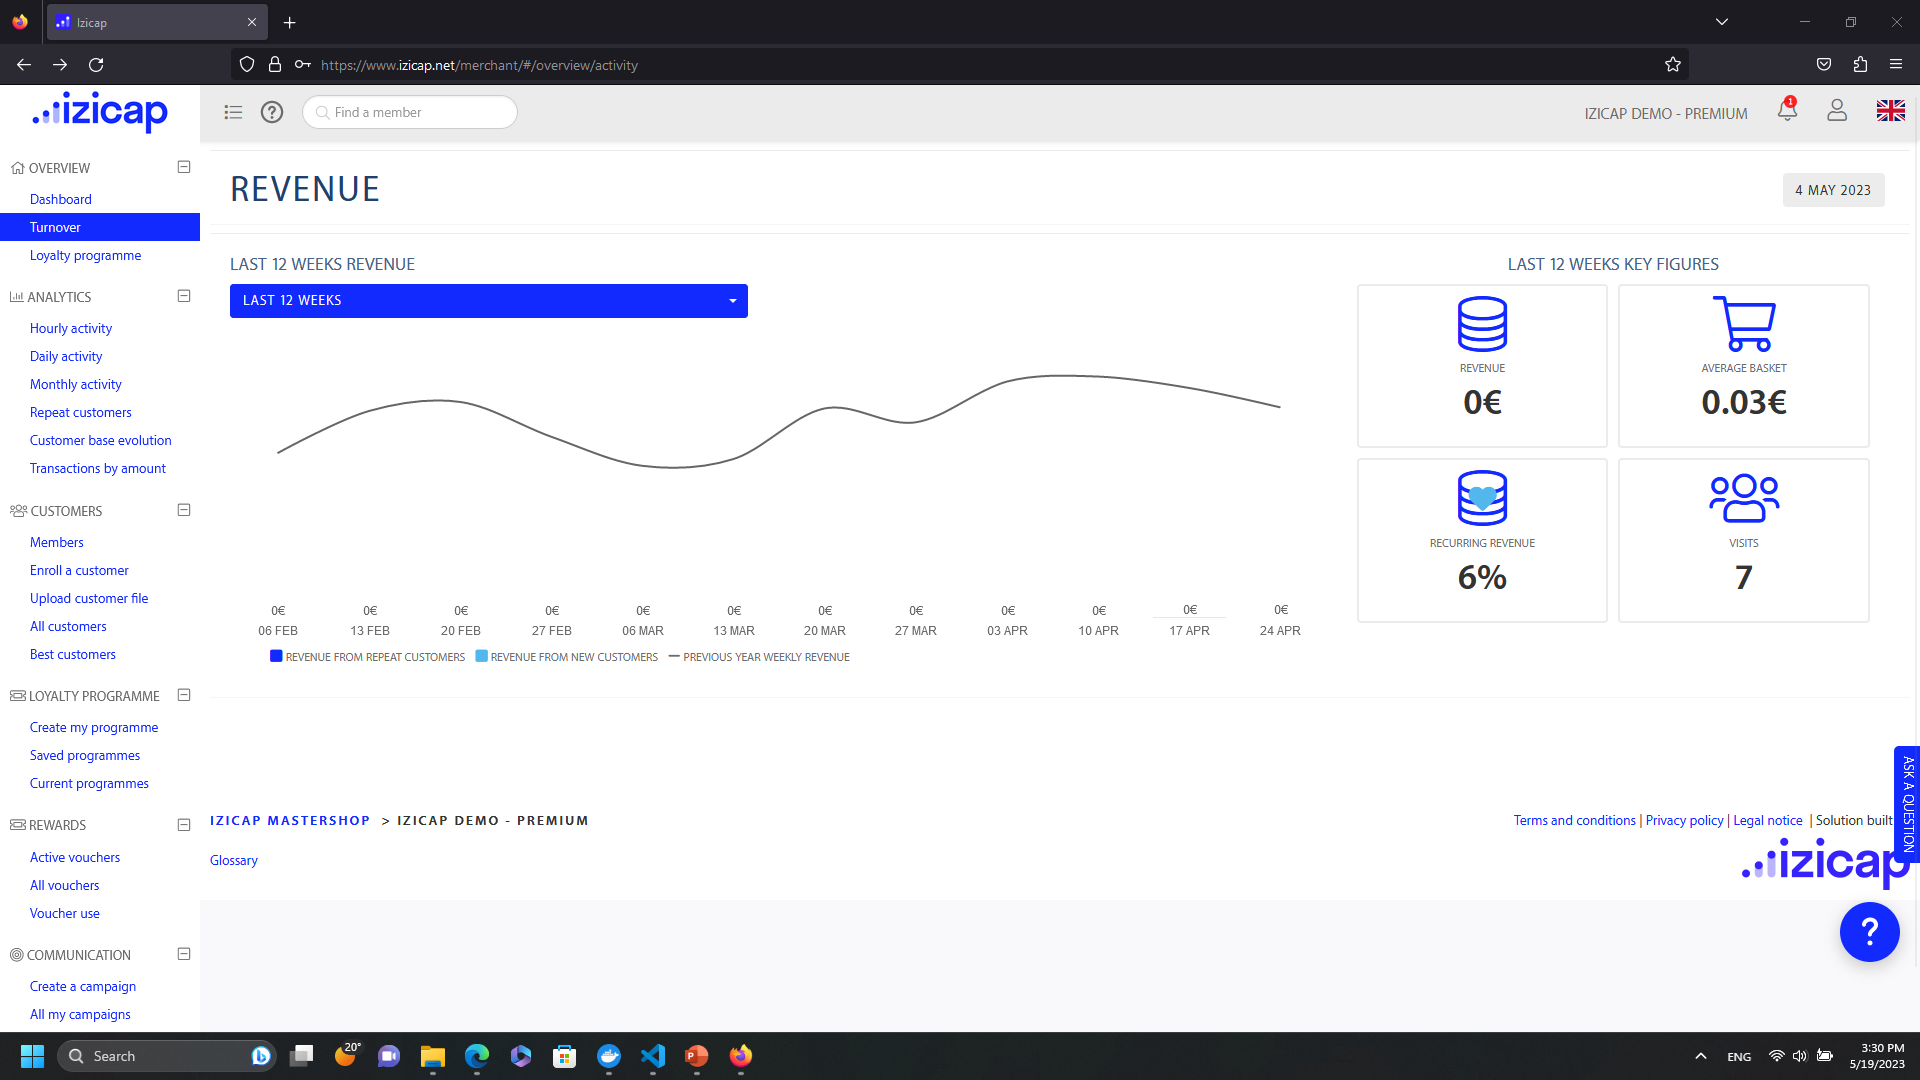
\includegraphics[width=\linewidth]{images/revenu.png}
\caption{Revenu des clients}\label{fig:izicap-2}
\end{figure}


\begin{figure}[H]
\centering
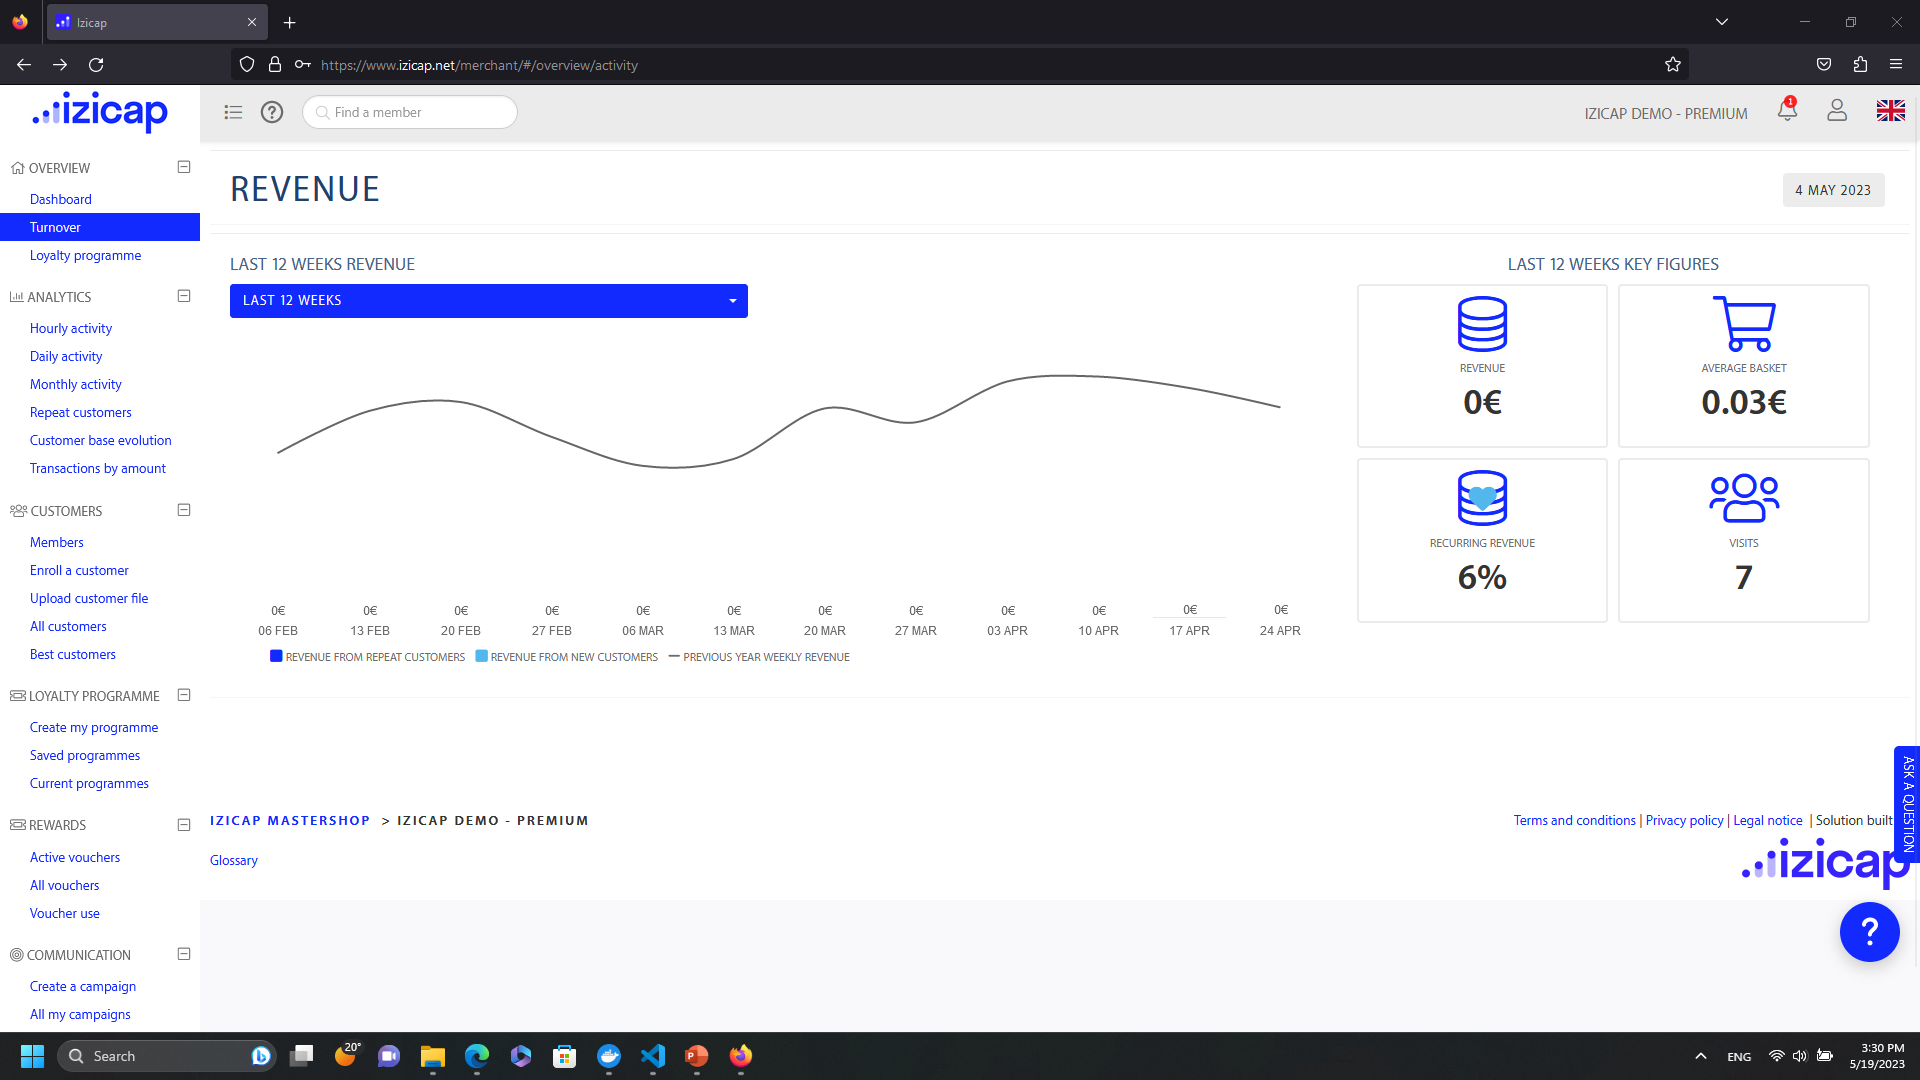
\includegraphics[width=\linewidth]{images/revenu.png}
\caption{Custommer base evolution}\label{fig:izicap-3}
\end{figure}
    
\begin{figure}[H]
\centering
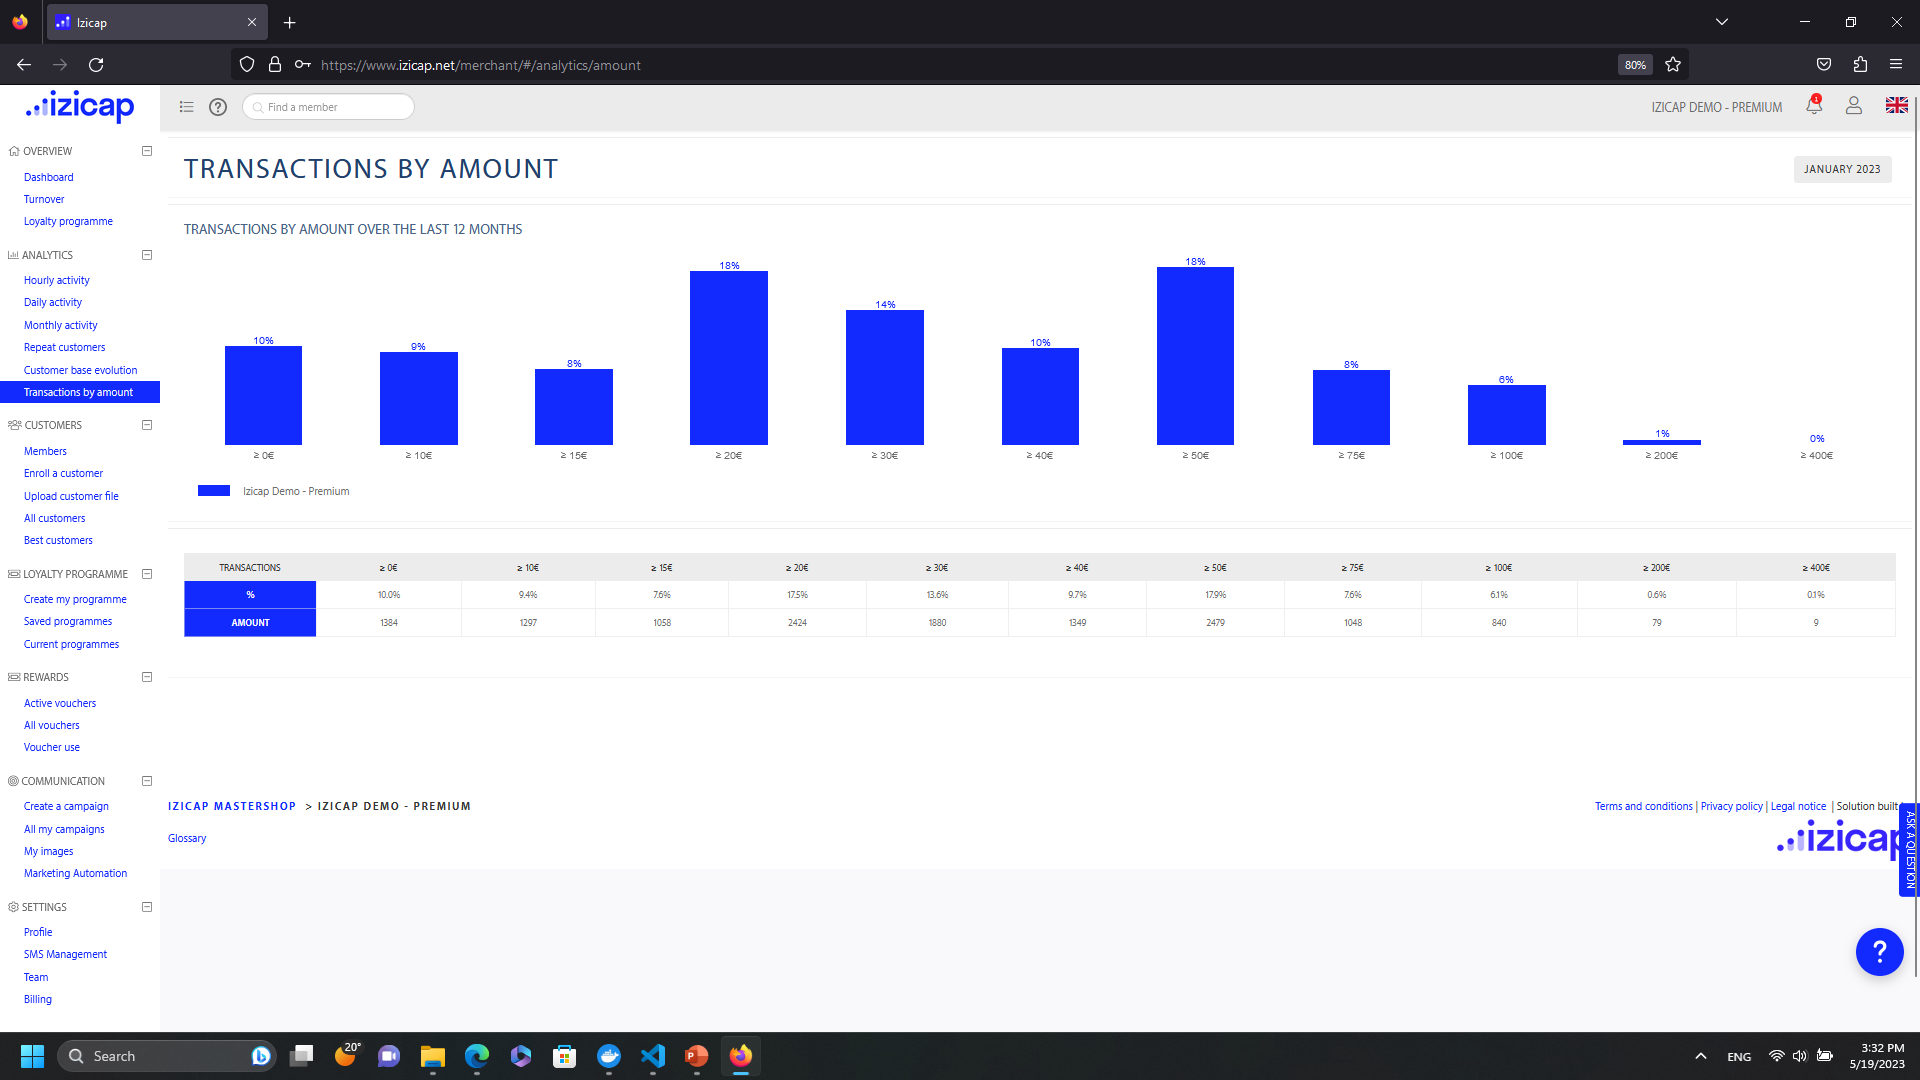
\includegraphics[width=\linewidth]{images/data-2.png}
\caption{Transactions by amount}\label{fig:izicap-4}
\end{figure}
        
L'utilisation des microfrontends permet de découper l'interface utilisateur en plusieurs modules indépendants, chacun étant responsable d'une fonctionnalité spécifique. Cela permet une séparation claire des responsabilités et facilite le développement, la maintenance et l'évolution de l'application.

\section*{Conclusion}
L'étude de faisabilité des connecteurs pour manipuler Delta Lake nous a permis de prendre des décisions éclairées sur l'implémentation de la solution. Bien que Spark soit largement utilisé et intégré à l'écosystème Big Data, Trino offre des avantages significatifs en termes de flexibilité et de performances pour les requêtes SQL. En fonction de nos besoins spécifiques et des contraintes techniques, nous avons opté pour l'utilisation de Trino comme connecteur pour manipuler Delta Lake dans notre solution.